%\documentclass[a4paper]{article}
%\usepackage[utf8]{inputenc}
\usepackage[spanish, es-tabla, es-noshorthands]{babel}
\usepackage[table,xcdraw,dvipsnames]{xcolor}
\usepackage[a4paper, footnotesep=1.25cm, headheight=1.25cm, top=2.54cm, left=2.54cm,
 bottom=2.54cm, right=2.54cm]{geometry}
%\geometry{showframe}
 \usepackage[normalem]{ulem}
 \useunder{\uline}{\ul}{}

%VERIFICAR EL HEAD Y EL FOOT EN
%https://ctan.dcc.uchile.cl/macros/latex/contrib/geometry/geometry.pdf

%Paquetes varios:
\usepackage{verbatimbox}

%\usepackage{wrapfig}			%Wrap figure in text
\usepackage[export]{adjustbox}	%Move images
\usepackage{changepage}			%Move tables
\usepackage{todonotes}

\usepackage{tikz}
\usepackage{amsmath}
\usepackage{amsfonts}
\usepackage{amssymb}
\usepackage{float}
\usepackage[graphicx]{realboxes}
\usepackage{caption}
\usepackage{subcaption}
\usepackage{multicol}
\usepackage{multirow}
\setlength{\doublerulesep}{\arrayrulewidth}
%\usepackage{booktabs}

\usepackage{array}
\newcolumntype{C}[1]{>{\centering\let\newline\\\arraybackslash\hspace{0pt}}m{#1}}
%\usepackage[american]{circuitikz}
\usetikzlibrary{calc}
\usepackage{fancyhdr}
\usepackage{units} 

\usepackage{colortbl}
%\usepackage{sectsty}
%\usepackage{unicode-math}

%FONTS (IMPORTANTE): Compilar en XeLaTex o LuaLaTeX
\usepackage{anyfontsize}	%Font size
\usepackage{fontspec}		%Font type
%Si sigue sin andar comentar \usepackage[utf8]{inputenc}
%https://ctan.dcc.uchile.cl/macros/unicodetex/latex/fontspec/fontspec.pdf
%https://www.overleaf.com/learn/latex/XeLaTeX

%Path para imagenes para trabajar en subarchivos
\graphicspath{{../Resumen/}{../Referencias/}{../Apendice/}{../Descripción de la Empresa/}{../Tareas del Alumno/}{../Conclusiones/}{../Herramientas Empleadas/}}

%Definiciones de nuevos comandos y colores
%COLORES:
\definecolor{AzulFoot}{rgb}{0.682,0.809,0.926}	%RGB	%{174,206,235}
\definecolor{AzulInfo}{rgb}{0.180,0.455,0.710}	%RGB	%{46,116,181}
\definecolor{AzulTable}{rgb}{0.302,0.507,0.871}	%RGB	%{68,114,196}
\definecolor{PName}{rgb}{0.353,0.353,0.353}		%RGB	%{90,90,90}
\definecolor{mygreen}{rgb}{28,172,0} % color values Red, Green, Blue
\definecolor{mylilas}{rgb}{170,55,241}

%Change Font Size

% #1 = size, #2 = text
\newcommand{\setparagraphsize}[2]{{\fontsize{#1}{6}\selectfont#2 \par}}		%Cambia el size de todo el parrafo
\newcommand{\setlinesize}[2]{{\fontsize{#1}{6}\selectfont#2}}				%Cambia el font de una oración

%IMAGE IN TABLE:			%Ejemplo: \includeintable{.3}{ImagenesFactibilidad/pend}
\renewcommand\fbox{\fcolorbox{white}{white}}
\setlength{\fboxrule}{0pt}	%padding thickness
\setlength{\fboxsep}{4pt}	%border thickness
\newcommand{\includeintable}[2]{	
	\fbox{
		\begin{minipage}{#1\textwidth}
        	\includegraphics[width=\linewidth]{#2}
    	\end{minipage}
	}
}

%LINK IN REF
\newcommand{\reflink}[1]{		%LINK
	\href{#1}{#1}
}

%NOTAS:
\newcommand{\note}[1]{		%RED BIG NOTE (TODO)
	\begin{center}
		\huge{ \textcolor{red}{#1} }
	\end{center}
}

\newcommand{\lnote}[1]{{\fontsize{14}{6}\selectfont\textcolor{green}{#1}}}	%Notas pequeñas

\newcommand{\observacion}[2]{  \ifnumequal{1}{#1}{ { \todo[inline,backgroundcolor=red!25,bordercolor=red!100]{\textbf{Observación: #2}} } }{  }  }

\newcommand{\red}[1]{\textcolor{red}{#1}}

\newcommand{\TBD}{\textcolor{red}{(TBD) }}
\newcommand{\tbd}{\textcolor{red}{(TBD) }}

\newcommand{\TBC}{\textcolor{red}{(TBC) }}
\newcommand{\tbc}{\textcolor{red}{(TBC) }}

\newcommand{\quotes}[1]{``#1''}
\newcommand{\q}[1]{``#1''}

\newcommand{\ip}{192.168.0.10:1880}
\newcommand{\ipadmin}{192.168.0.10:1880/admin}

% Comandos para agregar elementos en tablas de acronimos y definiciones
\newcommand{\addacronym}[2]{\textbf{#1} & \begin{tabular}[l]{@{}l@{}}#2\end{tabular} \\ \hline}

% tabItem
\newcommand{\tabitem}{~~\llap{\textbullet}~~}


\usepackage{hyperref}
\hypersetup{
    colorlinks=true,
    linkcolor=black,
    filecolor=magenta,      
    urlcolor=AzulInfo,
    citecolor=AzulInfo,    
}

%Configuración del header y del footer:
\usepackage{etoolbox}
\pagestyle{fancy}
\fancyhf{}
\rfoot{\thepage}
\renewcommand{\footrulewidth}{4pt}
\renewcommand{\headrulewidth}{0pt}
\patchcmd{\footrule}{\hrule}{\color{AzulFoot}\hrule}{}{}

%Código en el informe
%% IMPORTANTE:
% Verificar que esté \usepackage[dvipsnames]{xcolor}

%\usepackage{listingsutf8}
\usepackage{listings}

\renewcommand{\lstlistingname}{Código}

%LSTSET: Pone un recuadro y contador de linea en el codigo
\newcommand{\boxstyle}{
	\lstset{
		basicstyle=\sffamily\color{black},
		frame=single,
		numbers=left,
		numbersep=5pt,
		numberstyle=\color{gray},
		showspaces=false,
		showstringspaces=false
	}
}

\newcommand{\defaultstyle}{
	\lstset{
		basicstyle=\sffamily\color{white},
		frame=none,
		numbers=none,
		showspaces=true,
		showstringspaces=true
	}
}

\lstdefinelanguage{Kotlin}{
  captionpos=b,
  comment=[l]{//},
  commentstyle={\color{gray}\ttfamily},
  emph={filter, first, firstOrNull, forEach, lazy, map, mapNotNull, println},
  emphstyle={\color{OrangeRed}},
  identifierstyle=\color{black},
  keywords={!in, !is, abstract, actual, annotation, as, as?, break, by, catch, class, companion, const, constructor, continue, crossinline, data, delegate, do, dynamic, else, enum, expect, external, false, field, file, final, finally, for, fun, get, if, import, in, infix, init, inline, inner, interface, internal, is, lateinit, noinline, null, object, open, operator, out, override, package, param, private, property, protected, public, receiveris, reified, return, return@, sealed, set, setparam, super, suspend, tailrec, this, throw, true, try, typealias, typeof, val, var, vararg, when, where, while},
  keywordstyle={\color{NavyBlue}\bfseries},
  morecomment=[s]{/*}{*/},
  morestring=[b]",
  morestring=[s]{"""*}{*"""},
  ndkeywords={@Deprecated, @JvmField, @JvmName, @JvmOverloads, @JvmStatic, @JvmSynthetic, Array, Byte, Double, Float, Int, Integer, Iterable, Long, Runnable, Short, String, Any, Unit, Nothing},
  ndkeywordstyle={\color{BurntOrange}\bfseries},
  sensitive=true,
  stringstyle={\color{ForestGreen}\ttfamily},
}

\lstdefinelanguage{Swift}
{
  morekeywords={
    open,catch,@escaping,nil,throws,func,if,then,else,for,in,while,do,switch,case,default,where,break,continue,fallthrough,return,
    typealias,struct,class,enum,protocol,var,func,let,get,set,willSet,didSet,inout,init,deinit,extension,
    subscript,prefix,operator,infix,postfix,precedence,associativity,left,right,none,convenience,dynamic,
    final,lazy,mutating,nonmutating,optional,override,required,static,unowned,safe,weak,internal,
    private,public,is,as,self,unsafe,dynamicType,true,false,nil,Type,Protocol,
  },
  morecomment=[l]{//}, % l is for line comment
  morecomment=[s]{/*}{*/}, % s is for start and end delimiter
  morestring=[b]", % defines that strings are enclosed in double quotes
  breaklines=true,
  escapeinside={\%*}{*)},
  numbers=left,
  captionpos=b,
  breakatwhitespace=true,
  basicstyle=\linespread{1.0}\ttfamily, % https://tex.stackexchange.com/a/102728/129441
}

\definecolor{keyword}{HTML}{BA2CA3}
\definecolor{string}{HTML}{D12F1B}
\definecolor{comment}{HTML}{008400}

\newcommand{\swiftstyle}{
	\lstset{
  		language=Swift,
  		inputencoding=utf8x,
		extendedchars=\true,
	  	basicstyle=\ttfamily,
	  	showstringspaces=false, % lets spaces in strings appear as real spaces
  		columns=fixed,
  		keepspaces=true,
  		keywordstyle=\color{keyword},
  		stringstyle=\color{string},
  		commentstyle=\color{comment}
	}
}


%Como usarlo:

%\begin{lstlisting}[caption={Simple code listing.}, label={lst:example1}, language=Kotlin]
%// this is a simple code listing:
%println("hello kotlin from latex")
%\end{lstlisting}

%Si se corta en 2 páginas distintas:

%\vspace{1mm}
%\noindent{\begin{minipage}{\linewidth}
%\begin{lstlisting}[...]
%...
%\end{lstlisting}
%\end{minipage}}




\usepackage{titlesec}		%Para hacer las subsubsubsections

%Colores a los nombres de las secciones:
%\sectionfont{\color{AzulInfo}}  % sets color of sections
%\subsectionfont{\color{AzulInfo}}
%\subsubsectionfont{\color{AzulInfo}}

%PICTURES AND TABLE INDEX:
\newcommand{\Section}[1]{ \section{#1} 
	\phantomsection \setcounter{figure}{0} \setcounter{table}{0} \setcounter{lstlisting}{0}
		\renewcommand{\thetable}{\arabic{section}.\arabic{table}}
		\renewcommand{\thefigure}{\arabic{section}.\arabic{figure}}
		\renewcommand{\thelstlisting}{\arabic{section}.\arabic{lstlisting}}
}

\newcommand{\Subsection}[1]{ \subsection{#1}
	\phantomsection \setcounter{figure}{0} \setcounter{table}{0} \setcounter{lstlisting}{0}
		\renewcommand{\thetable}{\arabic{section}.\arabic{subsection}.\arabic{table}}
		\renewcommand{\thefigure}{\arabic{section}.\arabic{subsection}.\arabic{figure}}
		\renewcommand{\thelstlisting}{\arabic{section}.\arabic{subsection}.\arabic{lstlisting}}
}

\newcommand{\Subsubsection}[1]{ \subsubsection{#1} 
	\phantomsection \setcounter{figure}{0} \setcounter{table}{0}  \setcounter{lstlisting}{0}
		\renewcommand{\thetable}{\arabic{section}.\arabic{subsection}.\arabic{subsubsection}.\arabic{table}}
		\renewcommand{\thefigure}{\arabic{section}.\arabic{subsection}.\arabic{subsubsection}.\arabic{figure}}
		\renewcommand{\thelstlisting}{\arabic{section}.\arabic{subsection}.\arabic{subsubsection}.\arabic{lstlisting}}
}

%Definición de subsubsubsection:
\titleclass{\subsubsubsection}{straight}[\subsection]

\newcounter{subsubsubsection}[subsubsection]
\renewcommand\thesubsubsubsection{\thesubsubsection.\arabic{subsubsubsection}}

\titleformat{\subsubsubsection}
  {\normalfont\normalsize\bfseries\color{AzulInfo}}{\thesubsubsubsection}{1em}{}	%Color de subsubsubsection
\titlespacing*{\subsubsubsection}
{0pt}{3.25ex plus 1ex minus .2ex}{1.5ex plus .2ex}

\makeatletter
\renewcommand\paragraph{\@startsection{paragraph}{5}{\z@}%
  {3.25ex \@plus1ex \@minus.2ex}%
  {-1em}%
  {\normalfont\normalsize\bfseries}}
\renewcommand\subparagraph{\@startsection{subparagraph}{6}{\parindent}%
  {3.25ex \@plus1ex \@minus .2ex}%
  {-1em}%
  {\normalfont\normalsize\bfseries}}
\def\toclevel@subsubsubsection{4}
\def\toclevel@paragraph{5}
\def\toclevel@paragraph{6}
\def\l@subsubsubsection{\@dottedtocline{4}{7em}{4em}}
\def\l@paragraph{\@dottedtocline{5}{10em}{5em}}
\def\l@subparagraph{\@dottedtocline{6}{14em}{6em}}
\makeatother

\setcounter{secnumdepth}{4}
\setcounter{tocdepth}{4}

%Subsubsubsection:
\newcommand{\Subsubsubsection}[1]{ \subsubsubsection{#1} 
	\phantomsection \setcounter{figure}{0} \setcounter{table}{0} \renewcommand{\thetable}{\arabic{section}.\arabic{subsection}.\arabic{subsubsection}.\arabic{subsubsubsection}.\arabic{table}} \renewcommand{\thefigure}{\arabic{section}.\arabic{subsection}.\arabic{subsubsection}.\arabic{subsubsubsection}.\arabic{figure}}
}

%Tamaño, color e identación de sección, subsección, subsubsección y subsubsubsección:
%La identación de las subsecciones está tambien en Index-cfg.tex para el toc, lot y lot en el index
\titleformat{\section}[block]{\fontsize{16}{6}\selectfont\bfseries\color{AzulInfo}}{\thesection.}{1em}{} 
\titleformat{\subsection}[block]{\hspace{2.5em}\fontsize{13}{6}\selectfont\color{AzulInfo}}{\thesubsection}{1em}{}
\titleformat{\subsubsection}[block]{\hspace{3.5em}\fontsize{12}{6}\selectfont\color{AzulInfo}}{\thesubsubsection}{1em}{}
\titleformat{\subsubsubsection}[block]{\hspace{4em}\fontsize{11}{6}\selectfont\color{AzulInfo}}{\thesubsubsubsection}{1em}{}

%Pone las refrencias en el indice
\usepackage[numbib, nottoc, notlot, notlof]{tocbibind}

%Pone toc, lof y lot en colores y elijo el titulo de estos
\addto\captionsspanish{
	\renewcommand\contentsname{Contenidos}
	\renewcommand\listfigurename{Lista de Figuras}
	\renewcommand\listtablename{Lista de Tablas}
}

%Agrega TOC al indice
\renewcommand{\tableofcontents}{
	\stepcounter{section}
	\addcontentsline{toc}{section}{\protect\numberline{\thesection}\textbf{Contenidos}}
	\tableofcontents
}

%Agrega LOF al indice
\renewcommand{\listoffigures}{
	\stepcounter{section}
	\addcontentsline{toc}{section}{\protect\numberline{\thesection}\textbf{Lista de Figuras}}
	\listoffigures
}

%Agrega LOT al indice
\renewcommand{\listoftables}{
	\stepcounter{section}
	\addcontentsline{toc}{section}{\protect\numberline{\thesection}\textbf{Lista de Tablas}}
	\listoftables
}

%Indices: cambio la separación de los numeros para que entren tablas y fotos
\usepackage{tocloft}
\setlength{\cftfignumwidth}{1.35cm}  % change numwidth from figures in lof
\setlength{\cfttabnumwidth}{1.35cm}  % change numwidth from tables in lot
\renewcommand{\cfttoctitlefont}{\Large\bfseries\color{AzulInfo}}
\renewcommand{\cftloftitlefont}{\Large\bfseries\color{AzulInfo}}
\renewcommand{\cftlottitlefont}{\Large\bfseries\color{AzulInfo}}

%Coloca lineas punteadas a las seciones en el TOC
\renewcommand{\cftsecleader}{\cftdotfill{\cftdotsep}}

%Items con bullets y no cuadrados
\renewcommand{\labelitemi}{\textbullet }

%
%\def\verObs{1}
%\begin{document}

\Subsection{Factibilidad Tecnológica}

\Subsubsection{Esquema Modular}

A continuación se presentan los distintos módulos. Luego, en las siguientes subsecciones, se presentan las distintas alternativas evaluadas para la implementación.
\begin{figure}[H]
	\centering
	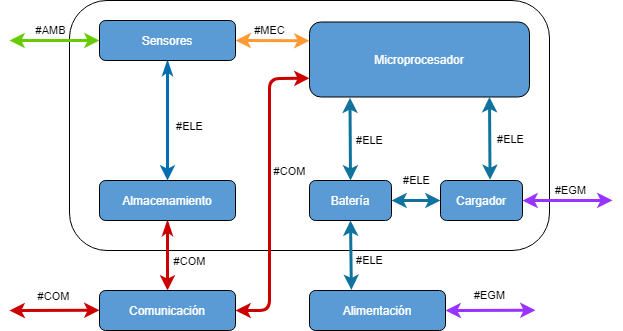
\includegraphics[width=0.9\linewidth]{ImagenesFactibilidad/EsquemaModular}
	\label{fig:esquema_modular}
	\caption{Diagrama modular del sistema.}
\end{figure}

\Subsubsection{Propuesta de Sensores}
Para las distintas mediciones se tuvieron en cuenta diversas tecnologías que existen. Se evaluaron parámetros que definen la performance, tales como la linealidad de salida, el costo, el rango de operación, la precisión, el tipo de salida, aplicación, entre otras tantas variables.

\Subsubsubsection{Temperatura}
En el caso de la medición de temperatura, se valoraron diversas tecnologías que existen, siendo por ejemplo la RTD cuyo funcionamiento se basa en el cambio de la resistencia en función de la temperatura bajo al ecuación $R(T)=R_0 + \alpha \cdot \Delta T$. También se consideró la tecnología TC, cuyo funcionamiento se basa en el \textit{efecto seebek}. Finalmente, el uso de un IC, el cual se basa en propiedades de dispositivos semiconductores extrínsecos.

\begin{table}[H]
\centering
\begin{tabular}{|c|c|c|c|c|}
\hline
\textbf{\begin{tabular}[c]{@{}c@{}}Aspectos\\ comparativos\end{tabular}} & \textbf{\href{https://www.thermocoupleinfo.com/type-k-thermocouple.htm}{TC-K}}                                                                             & \textbf{\href{http://www.datasheet.es/PDF/900325/Pt100-pdf.html}{PT-100}}                                                                                                              & \textbf{\href{https://datasheets.maximintegrated.com/en/ds/DS18B20.pdf}{Ds18b20}}                                                 & \textbf{\href{https://www.sparkfun.com/datasheets/Sensors/Temperature/DHT22.pdf}{DHT-22}}  \\ \hline
\textbf{Costo [ARS]}                                                           & 700	& 780	& 200	& 740	\\ \hline
\textbf{Tipo de salida}                                                  & Analógico                                                                                 & Analógico                                                                                                                    & Digital                                                          & Digital          \\ \hline

\textbf{\begin{tabular}[c]{@{}c@{}}Rango de\\ operación [°C]\end{tabular}}                                              & -40 $\sim$ 1200                                                                        & -50 $\sim$ 200  & -10 $\sim$ 85 & -40 $\sim$ 80 \\ \hline
\textbf{\begin{tabular}[c]{@{}c@{}}Interfaz de\\ conexionado\end{tabular}}                                                      & \begin{tabular}[c]{@{}c@{}}Se debe\\ proporcionar\\ un circuito\\ amplificador\end{tabular} & \begin{tabular}[c]{@{}c@{}}Se debe \\ proporcionar\\  un circuito\\  convertidor\\  de resistencia\\  a tensión\end{tabular} & -                                                                & -                \\ \hline
\textbf{Presición [°C]}                                                       & $\pm$ 1.5	& $\pm$ 0.1	& $\pm$ 0.5	& $\pm$ 0.5	\\ \hline

\textbf{Estabilidad}                                                     & Tienden a envejecer                                                                       & -                                                                                                                            & -                                                                & -                \\ \hline
\textbf{Autocalentamiento}                                               & -                                                                                         & \begin{tabular}[c]{@{}c@{}}Depende de\\  la corriente\\  de medición.\end{tabular}                                           & Bajo                                                             & Bajo             \\ \hline
\textbf{Imagen}                &  \includeintable{.1}{ImagenesFactibilidad/TC}                                                                                          &  \includeintable{.1}{ImagenesFactibilidad/PT100}                                                                                                                    & \includeintable{.1}{ImagenesFactibilidad/IC1}  &  \includeintable{.1}{ImagenesFactibilidad/DHT-22}                 \\ \hline
\end{tabular}
\caption{Comparación entre sensores de temperatura.}
\end{table}

\Subsubsubsection{Humedad}
Existen varias maneras de medir la magnitud física de la humedad, dentro de estas la mas común se basa en utilizar la dependencia que existe entre la humedad y la capacidad. Es por esto que se utilizan capacitores con un dieléctrico, el cual cambia constante con la humedad. Además existen sensores que se aprovechan de como cambia la resistencia en función de la temperatura, pero estas tecnologías son menos frecuentes.

\begin{table}[H]
\centering
\begin{tabular}{|c|c|c|c|c|}
\hline
\textbf{\begin{tabular}[c]{@{}c@{}}Aspectos\\ comparativos\end{tabular}} & \textbf{\href{https://www.mouser.com/datasheet/2/758/DHT11-Technical-Data-Sheet-Translated-Version-1143054.pdf}{DHT-11}}   & \textbf{\href{http://codigoelectronica.com/blog/am2301-datasheet}{AM-2301}}  & \textbf{\href{https://www.sparkfun.com/datasheets/Sensors/Temperature/DHT22.pdf}{DHT-22}}   & \textbf{\href{https://datasheetspdf.com/pdf/1298922/AOSONG/AM1001/1}{AM-1001}}  \\ \hline
\textbf{Costo [ARS]}                                                           & 200           & 1050 & 740 & 840	\\ \hline
\textbf{\begin{tabular}[c]{@{}c@{}}Rango de\\ operación [\%RH]\end{tabular}}                                              & 20 $\sim$ 90 & 0 $\sim$ 100 & 0 $\sim$ 100 & 20 $\sim$ 90 \\ \hline
\textbf{Presición [\%RH]}                                                       & $\pm$4	& $\pm$3	 & $\pm$2	& $\pm$5	\\ \hline
\textbf{Tipo de salida}                                                  & Digital           & Digital           & Digital           & Analógica         \\ \hline
\textbf{Imagen}                                                          & \includeintable{.1}{ImagenesFactibilidad/DHT-11}                 & \includeintable{.1}{ImagenesFactibilidad/AM-2301}                 & \includeintable{.1}{ImagenesFactibilidad/DHT-22}                 & \includeintable{.1}{ImagenesFactibilidad/AM-1001} \\ \hline
\end{tabular}
\caption{Comparación de sensores de humedad.}
\end{table}

\Subsubsubsection{Luminosidad}
En la medición del nivel de luminosidad se puede optar por diversos caminos. Existen sensores como el BH-1750 y OPT-100 que su funcionamiento se basa en un fotodiodo que conduce cierta corriente a partir de la luz que le impacta. Otros sensores, tales como el TEMT-600, emplean un fototransistor, cuya base se encuentra expuesta. En función de la intensidad lumínica en dicha zona, circulará cierta corriente por el colector. Finalmente existen fotoresistores, los cuales, tal como su nombre indica, cambian la resistencia en función del nivel de luz.
\begin{table}[H]
\centering
\begin{tabular}{|c|c|c|c|c|}
\hline
\textbf{\begin{tabular}[c]{@{}c@{}}Aspectos\\ comparativos\end{tabular}}              & \textbf{\href{https://www.mouser.com/datasheet/2/348/bh1750fvi-e-186247.pdf}{BH-1750}}  & \textbf{\href{https://www.vishay.com/docs/81579/temt6000.pdf}{TEMT-6000}}	& \textbf{\href{https://www.ti.com/lit/ds/symlink/opt101.pdf}{OPT-101}}                                              & \textbf{\href{https://www.alldatasheet.es/view.jsp?Searchword=GL55}{GL55-LM393}} \\ \hline
\textbf{Costo [ARS]}	& 230 	& 340	& 330	& 190	\\ \hline
\textbf{\begin{tabular}[c]{@{}c@{}}Rango de \\ temperatura\\  de operación [°C]\end{tabular}} & -40 $\sim$ 85  & -40 $\sim$ 85 & 0 $\sim$ 70 & -30 $\sim$ 70 \\ \hline
\textbf{\begin{tabular}[c]{@{}c@{}}Potencia\\ disipada [mW]\end{tabular}}                                                            & 260 	& 100 	& \TBD 	& 75 	\\ \hline
\textbf{Tipo de salida}                                                               & I2C               & \begin{tabular}[c]{@{}c@{}}Analógica\\ (Corriente)\end{tabular}                 & \begin{tabular}[c]{@{}c@{}}Analógica\\ (Tensión)\end{tabular} &\begin{tabular}[c]{@{}c@{}}Analógica \\ Digital\end{tabular}  \\ \hline
\textbf{Aplicación}                                                                   & -                 & \begin{tabular}[c]{@{}c@{}}Necesita un\\amplificador\\ de corriente\end{tabular} & -                                                             & -                   \\ \hline
\begin{tabular}[c]{@{}c@{}}\textbf{Tensión de} \\ \textbf{alimentación [V]} \end{tabular}                                                      & 4.5 	& \textless \ 6 	& 2.7 $\sim$ 36.0 	& 3.3 $\sim$ 5.0 	\\ \hline
\textbf{\begin{tabular}[c]{@{}c@{}}Rango de\\ medición [nm]\end{tabular}}                                                            & 450 $\sim$ 650 & 400 $\sim$ 900 & 450 $\sim$ 1000 & 450 $\sim$ 750 \\ \hline
\textbf{Imagen}                                                                       & \includeintable{.1}{ImagenesFactibilidad/BH-1750} & \includeintable{.1}{ImagenesFactibilidad/TEMT-6000}                                                                               & \includeintable{.1}{ImagenesFactibilidad/OPT-101} & \includeintable{.1}{ImagenesFactibilidad/GL55-LM393}                   \\ \hline
\end{tabular}
\caption{Comparación de sensores de luminosidad.}
\end{table}


\Subsubsubsection{Imagenes}
Para la obtención de imagenes y teniendo en cuenta la tecnología utilizada para la unidad de procesamiento, se encontraron diversos modulos de camara que se pueden usar:



\begin{table}[]
\centering
\begin{tabular}{|c|c|c|c|}
\hline
\textbf{\begin{tabular}[c]{@{}c@{}}Aspectos\\ comparativos\end{tabular}} & \textbf{RPi-CMOD-V1}             & \textbf{RPi-CMOD-V2}             & \textbf{Rpi-HQC}                 \\ \hline
\textbf{Costo}                                                           & 25 USD                           & 25 USD                           & 50 USD                           \\ \hline
\textbf{Tamaño {[}mm{]}}                                                 & 25x24x9                          & 25x24x9                          & 38x38x18.4                       \\ \hline
\textbf{Resolución camara}                                               & 5MP                              & 8MP                              & 12.3MP                           \\ \hline
\textbf{Integración Linux}                                               & V4L2 driver                      & V4L2 driver                      & V4L2 driver                      \\ \hline
\textbf{C API}                                                           & OpenMAX IL y otras               & OpenMAX IL y otras               & -                                \\ \hline
\textbf{Peso {[}g{]}}                                                    & 3                                & 3.4                              & 53                               \\ \hline
\textbf{Sensor}                                                          & OmniVision OV5647                & Sony IMX219                      & Sony IMX477                      \\ \hline
\multicolumn{1}{|l|}{\textbf{Rango de temperaturas °C}}                  & \multicolumn{1}{l|}{-25$\sim$80} & \multicolumn{1}{l|}{-25$\sim$80} & \multicolumn{1}{l|}{-25$\sim$80} \\ \hline
\textbf{Imagen}                                                          &  \includeintable{.1}{ImagenesFactibilidad/RPICAMV1}                    & \includeintable{.1}{ImagenesFactibilidad/RPICAMV2}                     & \includeintable{.1}{ImagenesFactibilidad/RPIHQCAM}                \\ \hline
\end{tabular}
\end{table}

\Subsubsection{Propuesta de Almacenamiento}
Para almacenar información, se considera la utilización memorias SD debido a su compacto tamaño comparado a la densidad de información que puede contener. Existe una gran variedad de memorias SD, permitiendo priorizar diversos aspectos a la hora de optar por una opción. La velocidad de lectura, la de escritura y el almacenamiento son algunos de estos aspectos, aunque en este proyecto también es importante considerar el rango de temperatura de operación.

\begin{table}[H]
\centering
\begin{tabular}{|c|c|c|c|}
\hline
\textbf{\begin{tabular}[c]{@{}c@{}}Aspectos\\ comparativos\end{tabular}}         & \textbf{\href{https://www.kingston.com/datasheets/sdcg3_es.pdf}{SDCG3}} & \textbf{\href{https://www.kingston.com/datasheets/mlpmr2_es.pdf}{SDCE}} & \textbf{\href{https://ar.mouser.com/datasheet/2/669/SanDisk_02052018_SDSDAF3_SDSDQAF3-1285144.pdf}{SDSDQAF3-XI}} \\ \hline
\textbf{Costo [USD]}                                                             & 20                                                        & 52 & 22                                                                                                 \\ \hline
\textbf{\begin{tabular}[c]{@{}c@{}}Temperatura de\\ operación [°C]\end{tabular}} & -25 $\sim$ 85                                                           & -25 $\sim$ 85                                                           & -40 $\sim$ 85                                                                                                    \\ \hline
\textbf{Almacenamiento [GB]}                                                     & 64 $\sim$ 512                                                           & 64 $\sim$ 256                                                           & 8 $\sim$ 128                                                                                                     \\ \hline
\textbf{\begin{tabular}[c]{@{}c@{}}Velocidad\\ R/W [MB/s]\end{tabular}}          & 170 / 90                                                                & 285 / 165                                                               & 50 / 80                                                                                                          \\ \hline
\textbf{Alimentación [V]}                                                        & 3.3                                                                     & 3.3                                                                     & 2.7 $\sim$ 3.6                                                                                                   \\ \hline
\textbf{Imagen}                                                                  & \includeintable{.1}{ImagenesFactibilidad/SDCG3}                         & \includeintable{.1}{ImagenesFactibilidad/SDCE}                          & \includeintable{.1}{ImagenesFactibilidad/SDSDQAF3}                                                               \\ \hline
\end{tabular}
\caption{Comparación entre memorias SD.}
\end{table}

%\Subsubsection{Propuesta de Comunicación}
%En cuanto a la comunicación se utilizará BLE para la conexión con el ave, y WiFi para la comunicación con un tercero.
Ambos de estos se encuentran disponibles para su uso en el módulo Raspberry Pi Zero W.

\Subsubsection{Propuesta de Unidad de Procesamiento}
\label{sec:antenas}
La UP representa el cerebro del proyecto. Este se ocupa de procesar la información de los sensores, almacenarla en la SD e iniciar los procesos de comunicación. En otras palabras, el integrado se ocupa de conectar los distintos módulos entre sí y garantizar su adecuado funcionamiento.

\begin{table}[H]
\centering
\begin{tabular}{|c|c|c|c|}
\hline
\textbf{\begin{tabular}[c]{@{}c@{}}Aspectos\\ comparativos\end{tabular}}         & \textbf{\href{https://datasheets.raspberrypi.org/rpi4/raspberry-pi-4-product-brief.pdf}{RPi 4}} & \textbf{\href{https://www.raspberrypi.org/products/raspberry-pi-zero-w/}{RPi Zero W}}            		& \href{https://static.raspberrypi.org/files/product-briefs/Raspberry-Pi-Model-Bplus-Product-Brief.pdf}{RPi 3B} 	\\ \hline
\textbf{Costo [USD]}                                                             & 55                                                                              & 25.5 		& 100 	\\ \hline
\textbf{\begin{tabular}[c]{@{}c@{}}Temperatura de\\ operación [°C]\end{tabular}} & 0 $\sim$ 50                                                                                     & -20 $\sim$ 85 																							& -20 $\sim$ 85                                                                                                                                                                                                      	\\ \hline
\textbf{Memoria}                                                            	 & 1 [GB] $\sim$ 8 [GB]                                                                            & 512 [MB]                                                                                             	& 1 [GB] $\sim$ 8 [GB]                                                                                                                                                                                                  \\ \hline
\textbf{Conexiones}                                                              & \begin{tabular}[c]{@{}c@{}}Wireless LAN,\\ Bluetooth 5.0,\\ Ethernet, USB\end{tabular}          & \begin{tabular}[c]{@{}c@{}}Wireless LAN,\\ Bluetooth 4.1 (BLE),\\ Micro USB, mini HDMI\end{tabular} 	& \begin{tabular}[c]{@{}c@{}}Wireless LAN,\\ Bluetooth 5.0 (BLE),\\ Ethernet, USB,\\ antena externa\end{tabular}                                                                                                        \\ \hline
\textbf{Sonido y video}                                                          & \begin{tabular}[c]{@{}c@{}}Micro HDMI,\\ MIPI DSI y CSI\end{tabular}                            & \begin{tabular}[c]{@{}c@{}}Mini HDMI, HDMI,\\ CSI, PAL/NTSC pads\end{tabular}                   		& \begin{tabular}[c]{@{}c@{}}HDMI, MIPI DSI\\ y CSI, SDIO\end{tabular}                                                                                                                                               	\\ \hline
\textbf{Soporte SD}                                                              & \begin{tabular}[c]{@{}c@{}}Almacenamiento y\\ carga de SO\end{tabular}                          & Micro SD                                                                                        		& \begin{tabular}[c]{@{}c@{}}Entrada SD para tarjeta\\ o eMMC externo\end{tabular}                                                                                                                                   	\\ \hline
\textbf{Dimensiones [mm]}                                                        & 85.6 x 56.5                                                                                     & 65 x 30                                                                                         		& 40 x 55 																																																				\\ \hline
\textbf{Alimentación}                                                            & 5 V (3 A)                                                                                       & 5 (1.2 A)                                                                                       		& 5 V (1.4 A)                                                                                                                                                                                                        	\\ \hline
\textbf{Imagen}                                                                  & \includeintable{.1}{ImagenesFactibilidad/RPI4}                                   			   & \includeintable{.1}{ImagenesFactibilidad/RPIZero}                                						& \includeintable{.1}{ImagenesFactibilidad/RPICM}                                                                                                                                                                    	\\ \hline
\end{tabular}
\caption{Comparación entre placas \rspi.}
\label{comp:Rpi}
\end{table}

%\lnote{Creo que el procesador de todas va más o menos de -40 °C a 85 °C, pero las demás cosas lo limitan, por ejemplo el modulo de LAN creo que no va menos de 0 °C.}

%https://copperhilltech.com/content/The%20Operating%20Temperature%20For%20A%20Raspberry%20Pi%20%E2%80%93%20Technologist%20Tips.pdf

\Subsubsection{Propuesta de Batería}
Para la elección de las baterías, se evaluaron unidades de tecnología de gel de carga profunda.

\begin{table}[H]
\centering
\begin{tabular}{|c|c|c|c|c|}
\hline
\textbf{\begin{tabular}[c]{@{}c@{}}Aspectos\\ comparativos\end{tabular}}                          & \textbf{\begin{tabular}[c]{@{}c@{}}\href{https://www.kijo-battery.com/products/jdg-series-agm-gel-deep-cycle-battery.html}{Kijo Serie}\\ \href{https://www.kijo-battery.com/products/jdg-series-agm-gel-deep-cycle-battery.html}{JDG}\end{tabular}} & \textbf{\begin{tabular}[c]{@{}c@{}}\href{https://www.kijo-battery.com/products/jlg-series-pure-gel-deep-cycle-battery.html}{Kijo Serie}\\ \href{https://www.kijo-battery.com/products/jlg-series-pure-gel-deep-cycle-battery.html}{JLG}\end{tabular}} & \textbf{\begin{tabular}[c]{@{}c@{}}\href{http://www.fenk.com.ar/wp-content/uploads/2020/01/JS12-20-1.pdf}{Fenk}\\ \href{http://www.fenk.com.ar/wp-content/uploads/2020/01/JS12-20-1.pdf}{JS12-20}\end{tabular}} & \textbf{\begin{tabular}[c]{@{}c@{}}\href{http://www.fenk.com.ar/productos/energias-renovables/baterias-solares/}{Fenk Serie}\\ \href{http://www.fenk.com.ar/productos/energias-renovables/baterias-solares/}{JM12}\end{tabular}} \\ \hline
\textbf{Costo [ARS]}                                                                              & 30500 $\sim$ X                                                                                                                                                                                                                                      & -                                                                                                                                                                                                                                            			& 6365 $\sim$ 8744                                                                                                                                                                                                & 20332 $\sim$ 76110                                                                                                                                                                                                               \\ \hline
\textbf{\begin{tabular}[c]{@{}c@{}}Temperatura de\\ operación [°C]\end{tabular}}                  & -20 $\sim$ 50                                                                                                                                                                                                                                       & -20 $\sim$ 50                                                                                                                                                                                                                                         & -20 $\sim$ 50                                                                                                                                                                                                   & -20 $\sim$ 50                                                                                                                                                                                                                    \\ \hline
\textbf{\begin{tabular}[c]{@{}c@{}}Tensión\\ nominal [V]\end{tabular}}                            & 12                                                                                                                                                                                                                                                  & 12                                                                                                                                                                                                                                                    & 12                                                                                                                                                                                                              & 12                                                                                                                                                                                                                               \\ \hline
\textbf{Capacidad [Ah]}                                                                           & 33 $\sim$ 250                                                                                                                                                                                                                                       & 100 $\sim$ 200                                                                                                                                                                                                                                        & 13.2 $\sim$ 20.0                                                                                                                                                                                                & 32.7 $\sim$ 200.0                                                                                                                                                                                                                \\ \hline
\textbf{\begin{tabular}[c]{@{}c@{}}Dimensiones\\ (máximas) [mm]\end{tabular}}                     & 52 x 268 x 220                                                                                                                                                                                                                                      & 499 x 259 x 219                                                                                                                                                                                                                                       & 181 x 77 x 167                                                                                                                                                                                                  & 522 x 240 x 219                                                                                                                                                                                                                  \\ \hline
\textbf{Peso [kg]}                                                                                & 10 $\sim$ 61                                                                                                                                                                                                                                        & 30 $\sim$ 74                                                                                                                                                                                                                                          & 5.45                                                                                                                                                                                                            & 15.5 $\sim$ 57.0                                                                                                                                                                                                                 \\ \hline
\textbf{\begin{tabular}[c]{@{}c@{}}Porcentaje de\\ autodescarga\\ (mensual a 25 °C)\end{tabular}} & 3\%                                                                                                                                                                                                                                                 & 3\%                                                                                                                                                                                                                                                   & 3\%                                                                                                                                                                                                             & 3\%                                                                                                                                                                                                                              \\ \hline
\textbf{Imagen}                                                                                   & \includeintable{.1}{ImagenesFactibilidad/Kijo-JDG}                                                                                                                                                                                                  & \includeintable{.1}{ImagenesFactibilidad/Kijo-JLG}                                                                                                                                                                                                    & \includeintable{.1}{ImagenesFactibilidad/Fenk-JS12-20}                                                                                                                                                          & \includeintable{.1}{ImagenesFactibilidad/Fenk-JM12}                                                                                                                                                                              \\ \hline
\end{tabular}
\caption{Comparación entre baterías gel de carga profunda.}
\end{table}

\Subsubsection{Propuesta de Alimentación}
\input{../Factibilidad/Tecnologica/Alimentación.tex}

\Subsubsection{Primer Propuesta de Abastecimiento de Energía de UBM}
\begin{table}[H]
\centering
\begin{tabular}{|c|c|c|c|}
\hline
\textbf{\begin{tabular}[c]{@{}c@{}}Aspectos\\ comparativos\end{tabular}}    & \href{https://abracon.com/patchantenna/APAE915R2540ABDB1-T.pdf}{APAE915R2540ABDB1-T} & \href{https://www.digikey.com/en/products/detail/pulselarsen-antennas/W3215/9838686}{W3215} & \href{https://cdn.taoglas.com/datasheets/ISPC.91A.09.0092E.pdf}{ISPC.91A.09.0092E} \\ \hline
\textbf{Dimensiones [mm]}                                                   & 25 x 25 x 4                                                                          & 40 x 40 x 6                                                                                 & 47 x 47 x 6.5                                                                      \\ \hline
\textbf{\begin{tabular}[c]{@{}c@{}}Frecuencia\\ Central [MHz]\end{tabular}} & 915                                                                                  & 915                                                                                         & 915                                                                                \\ \hline
\textbf{Impedancia [$\Omega$]}                                              & 50                                                                                   & 50                                                                                          & 50                                                                                 \\ \hline
\textbf{Polarización}                                                       & RHCP                                                                                 & Lineal vertical                                                                             & RHCP                                                                               \\ \hline
\textbf{Ganancia [dBi]}                                                     & 1.5                                                                                  & 4.5                                                                                         & 5 (30 x 30 ground plane)                                                           \\ \hline
\textbf{ROE}                                                                & 1.5                                                                                  & 1.23                                                                                        & 1.28                                                                               \\ \hline
\textbf{Costo [USD]}                                                        & 3.66                                                                                 & 12.47                                                                                       & 20.91                                                                              \\ \hline
\textbf{Imagen}                                                             & \includeintable{.1}{ImagenesFactibilidad/ANT1}                                       & \includeintable{.1}{ImagenesFactibilidad/ANT2}                                              & \includeintable{.1}{ImagenesFactibilidad/ANT3}                                     \\ \hline
\textbf{Lóbulo}                                                             & \includeintable{.1}{ImagenesFactibilidad/LOB1}                                       & \includeintable{.1}{ImagenesFactibilidad/LOB2}                                              & \includeintable{.1}{ImagenesFactibilidad/LOB3}                                     \\ \hline
\end{tabular}
\caption{Comparación entre antenas transmisoras (Parte 1).}
\end{table}

\begin{table}[H]
\centering
\begin{tabular}{|c|c|c|}
\hline
\textbf{\begin{tabular}[c]{@{}c@{}}Aspectos\\ comparativos\end{tabular}}    & \href{https://abracon.com/patchantenna/APAES915R80C16-T.pdf}{APAES915R80C16-T} & \href{https://abracon.com/datasheets/ARRKP7059-S915B.pdf}{ARRKP7059-S915B} \\ \hline
\textbf{Dimensiones [mm]}                                                   & 80 x 80 x 6                                                                    & 70 x 70 x 5.9                                                              \\ \hline
\textbf{\begin{tabular}[c]{@{}c@{}}Frecuencia\\ Central [MHz]\end{tabular}} & 915                                                                            & 915                                                                        \\ \hline
\textbf{Impedancia [$\Omega$]}   											& 50                                                                             & 50                                                                         \\ \hline
\textbf{Polarización}                                                       & RHCP                                                                           & RHCP                                                                       \\ \hline
\textbf{Ganancia [dBi]}                                                     & 2 (120 x 120 ground plane)                                                     & 2.8 (70 x 70 ground plane)                                                 \\ \hline
\textbf{ROE}                                                                & 1.3                                                                            & $\leq$ 2                                                                   \\ \hline
\textbf{Costo [USD]}                                                        & 34.28                                                                          & 50.73                                                                      \\ \hline
\textbf{Imagen}                                                             & \includeintable{.1}{ImagenesFactibilidad/ANT4}                                 & \includeintable{.1}{ImagenesFactibilidad/ANT5}                             \\ \hline
\textbf{Lóbulo}                                                             & \includeintable{.1}{ImagenesFactibilidad/LOB4}                                 & \includeintable{.1}{ImagenesFactibilidad/LOB5}                             \\ \hline
\end{tabular}
\caption{Comparación entre antenas transmisoras (Parte 2).}
\end{table}

\begin{table}[H]
\centering
\begin{tabular}{|c|c|c|c}
\hline
\textbf{\begin{tabular}[c]{@{}c@{}}Aspectos\\ comparativos\end{tabular}}    & \textbf{\href{https://linxtechnologies.com/wp/wp-content/uploads/ant-915-cpa-ds.pdf}{ANT-915-CPA}} & \textbf{\href{https://cdn.taoglas.com/datasheets/FXP290.07.0100A.pdf}{FXP290.07.0100A}} & \multicolumn{1}{c|}{\textbf{\href{https://media.digikey.com/pdf/Data\%20Sheets/Ignion\%20PDFs/NN01-105_Jan2021.pdf}{NN01-105}}} 	\\ \hline
\textbf{Dimensiones [mm]}                                                   & 25 x 25 x 4                                                                                        & 70 x 45 x 0.1                                                                           & \multicolumn{1}{c|}{18 x 7.3 x 0.8}                                                                                             	\\ \hline
\textbf{\begin{tabular}[c]{@{}c@{}}Frecuencia\\ Central [MHz]\end{tabular}} & 915                                                                                                & 915                                                                                     & \multicolumn{1}{c|}{915}                                                                                                      		\\ \hline
\textbf{Impedancia [$\Omega$]}                                              & 50                                                                                                 & 50                                                                                      & \multicolumn{1}{c|}{50} 		                                                                                                    \\ \hline
\textbf{Polarización}                                                       & RHCP                                                                                               & Lineal                                                                                  & \multicolumn{1}{c|}{Lineal}    		                                                                                            \\ \hline
\textbf{Ganancia [dBi]}                                                     & 1.5                                                                                                & 0.5                                                                                     & \multicolumn{1}{c|}{1.7}               		                                                                                    \\ \hline
\textbf{Eficiencia [\%]}                                                    & 38                                                                                                 & 43                                                                                      & \multicolumn{1}{c|}{85}                        	  	                                                                            \\ \hline
\textbf{ROE}                                                                & $\leq$ 1.2                                                                                           & 1.5                                                                                     & \multicolumn{1}{c|}{1.4}                               		                                                                    \\ \hline
\textbf{Costo [USD]}                                                       	& 3.9                                                                                                & 15.39                                                                                   & \multicolumn{1}{c|}{3.53}                                      		                                                            \\ \hline
\textbf{Peso [gr]}                                                          & 13.2                                                                                               & 1.5                                                                                     & 0.2                                                                    		                                                    \\ \hline
\textbf{Imagen}                                                             & \includeintable{.1}{ImagenesFactibilidad/ANTR1}                                                    & \includeintable{.1}{ImagenesFactibilidad/ANTR2}                                         & \multicolumn{1}{c|}{\includeintable{.1}{ImagenesFactibilidad/ANTR3}}           		                                            \\ \hline
\textbf{Lóbulo}                                                             & \includeintable{.1}{ImagenesFactibilidad/LOBR1}                                                    & \includeintable{.1}{ImagenesFactibilidad/LOBR2}                                         & \multicolumn{1}{c|}{"Omnidireccional"}                                                 		                                    \\ \hline
\end{tabular}
\caption{Comparación entre antenas receptoras (Parte 1).}
\end{table}

\begin{table}[H]
\centering
\begin{tabular}{|c|c|c|c}
\hline
\textbf{\begin{tabular}[c]{@{}c@{}}Aspectos\\ comparativos\end{tabular}}    & \textbf{\href{https://www.yageo.com/upload/media/product/productsearch/datasheet/wireless/An_SMD_FR4_915M_1204_05.pdf}{ANT1204F005R0915A}} & \textbf{\href{https://www.te.com/commerce/DocumentDelivery/DDEController?Action=srchrtrv&DocNm=1513156&DocType=DS&DocLang=English}{1513156-1}} & \multicolumn{1}{c|}{\textbf{\href{https://linxtechnologies.com/wp/wp-content/uploads/ant-915-usp410-ds.pdf}{ANT-915-USP410}}} \\ \hline
\textbf{Dimensiones [mm]}                                                   & 12.20 x 4 x 1.6                                                                                                                            & 38.1 x 6.6 x 1.57                                                                                                                              & \multicolumn{1}{c|}{13.2 x 9.1 x 2.9}                                                                                         \\ \hline
\textbf{\begin{tabular}[c]{@{}c@{}}Frecuencia\\ Central [MHz]\end{tabular}} & 915                                                                                                                                        & 915                                                                                                                                            & \multicolumn{1}{c|}{915}                                                                                                      \\ \hline
\textbf{Impedancia [$\Omega$]}                                              & 50                                                                                                                                         & 50                                                                                                                                             & \multicolumn{1}{c|}{50}                                                                                                       \\ \hline
\textbf{Polarización}                                                       & Lineal                                                                                                                                     & Lineal                                                                                                                                         & \multicolumn{1}{c|}{Lineal}                                                                                                   \\ \hline
\textbf{Ganancia [dBi]}                                                     & 1.59                                                                                                                                       & 1                                                                                                                                              & \multicolumn{1}{c|}{0}                                                                                                        \\ \hline
\textbf{Eficiencia [\%]}                                                    & -                                                                                                                                          & 88                                                                                                                                             & \multicolumn{1}{c|}{27}                                                                                                       \\ \hline
\textbf{ROE}                                                                & -                                                                                                                                          & 1.85                                                                                                                                           & \multicolumn{1}{c|}{1.5}                                                                                                      \\ \hline
\textbf{Costo [USD]}                                                       	& 1.52                                                                                                                                       & 2.8                                                                                                                                            & \multicolumn{1}{c|}{1.45}                                                                                                     \\ \hline
\textbf{Peso [gr]}                                                          & -                                                                                                                                          & < 0.9                                                                                                                                          & 0.6                                                                                                                           \\ \hline
\textbf{Imagen}                                                             & \includeintable{.1}{ImagenesFactibilidad/ANTR4}                                                                                            & \includeintable{.1}{ImagenesFactibilidad/ANTR5}                                                                                                & \multicolumn{1}{c|}{\includeintable{.1}{ImagenesFactibilidad/ANTR6}}                                                          \\ \hline
\textbf{Lóbulo}                                                             & \includeintable{.1}{ImagenesFactibilidad/LOBR4}                                                                                            & \includeintable{.1}{ImagenesFactibilidad/LOBR5}                                                                                                & \multicolumn{1}{c|}{\includeintable{.1}{ImagenesFactibilidad/LOBR6}}                                                          \\ \hline
\end{tabular}
\caption{Comparación entre antenas receptoras (Parte 2).}
\end{table}
\Subsubsection{Propuesta Final de Abastecimiento de Energía de UBM}
Ante la imposibilidad de realizar la carga inalámbrica se tuvo una reunión con el cliente para discutir el proceder. El cliente indicó que el dato principal que se requiere del ave es la posición. Para la obtención de datos de la trayectoria del ave se propuso el esquema que se explica a continuación.

\Subsubsubsection{Módulos del Sistema de Seguimiento}
La propuesta se basa en cuatro partes: la mochila en el ave, las bases de seguimiento, la base principal de seguimiento y la comunicación de esta con la base del nido. 
\begin{figure}[H]
	\centering
	\minipage{0.5\textwidth}
    	\centering
    	\includegraphics[width=\linewidth, page=1]{ImagenesFactibilidad/beacon}
    	\caption{Base de seguimiento.}
    \endminipage\hfill
    \minipage{0.5\textwidth}
    	\centering
    	\includegraphics[width=\linewidth, page=2]{ImagenesFactibilidad/beacon}
    	\caption{Base principal de seguimiento.}
    \endminipage	\\
    \minipage{0.5\textwidth}
    	\centering
    	\includegraphics[width=\linewidth, page=3]{ImagenesFactibilidad/beacon}
    	\caption{Base Nido.}
    \endminipage\hfill
    \minipage{0.5\textwidth}
    	\centering
    	\includegraphics[width=\linewidth,page=4]{ImagenesFactibilidad/beacon}
    	\caption{Mochila.}
    \endminipage
	\caption{Elementos ilustrativos de los módulos del sistema de seguimiento.}
	\label{fig:componentes_beacon_ilustrativo}
\end{figure}

\Subsubsubsection{Mochila}
Para la propuesta de la mochila, se llegó a la conclusión de que utilizar GPS es muy costoso en materia de energía, peso y dimensiones. Es por esto que tomó un camino alternativo, recomendando la tecnología de Beacon Bluetooth.

Se toma como ejemplo el modelo de beacon EMBC22, cuyas dimensiones son útiles para la aplicación deseada, dado que miden 30 $mm$ de diámetro y 10 $mm$ de altura. Junto a la batería se llega a un peso de 10 gramos, cumpliendo así con los requerimientos de dimensiones y de peso estipulados.

La característica más notable del beacon es que permite mandar paquetes personalizables por Bluetooth 5.0 a bases receptoras para informar su presencia. A partir estas se puede obtener la ubicación. Además este dispositivo soporta un amplio rango de temperaturas y cuenta con un grado de protección IP-64.

Para garantizar el funcionamiento durante todo el período del estudio se calcula una vida útil de la batería{Se utiliza la calculadora de vida útil del proveedor del beacon.}. Con un rango de detección de hasta 200 metros y un microcontrolador con acelerómetro y firmware personalizable, se obtiene un valor de 4 años.
\begin{figure}[H]
	\centering
	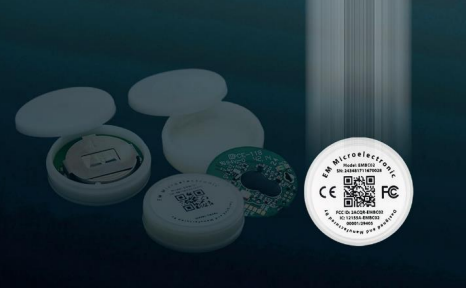
\includegraphics[width=0.7\linewidth]{ImagenesFactibilidad/beaconpic}
	\caption{Beacon EMBC22.}
	\label{fig:beacon}
\end{figure}

\Subsubsubsection{Base de Seguimiento}
Las bases de seguimiento consisten en una red de módulos receptores esparcidos por el bosque a una distancia de aproximadamente 30 metros entre sí.
Además, se hicieron las siguientes recomendaciones:
\begin{itemize}
	\item Comunicación Bluetooth 5.0 para el beacon acorde al estándar, con la finalidad de poder triangular su posición.
	\item Uso de red Lora o Bluetooth 5.0 para la comunicación entre bases de seguimiento de ser necesario y con la base principal de seguimiento para reporte de datos.
	\item Uso de paneles solares y baterías para lograr independencia de la red eléctrica.
\end{itemize}
\begin{figure}[H]
\centering
	\minipage{0.5\textwidth}
    	\centering
    	\includegraphics[width=\linewidth,page=5]{/ImagenesFactibilidad/beacon}
  		\caption{Ubicación de bases de seguimiento.}
  		\label{fig:sfig1}
    \endminipage\hfill
    \minipage{0.5\textwidth}
    	\centering
    	\includegraphics[width=\linewidth,page=6]{/ImagenesFactibilidad/beacon}
  		\caption{Triangulación de posición.}
  		\label{fig:sfig2}
    \endminipage
	\caption{Elementos ilustrativos de los módulos del sistema de seguimiento.}
	\label{fig:componentes beacon}
\end{figure}

\Subsubsubsection{Base Principal de Seguimiento}
La base principal de seguimiento junta toda la información de las demás centrales. Se considera la existencia de repetidores, los cuales son empleados para la señal del módulo principal. Esto permite extender la distancia en el caso de que la red receptora se encuentre fuera de alcance de la principal.

Dicha base también debe contar con independencia de la red eléctrica, y debe poder comunicarse con la del nido mediante Bluetooth. El propósito de esta comunicación es el enviar un set de datos del ave una vez por día.

\Subsubsubsection{Propuesta de Valor Aumentada}
Se destaca que al realizar el diseño sugerido, aumenta con creces la modularidad del producto final. Con la red de receptores desplegada, es posible escalar el sistema para más de un animal a la vez. Esto es posible simplemente con utilizar un beacon en las especies que se deseen seguir. 

Debido a la nivel de configuración que estos poseen, se puede distinguir a los distintos dispositivos entre sí, creando así un bosque inteligente para el seguimiento de toda su fauna.


\Subsubsection{Elección de una Solución}
\Subsubsubsection{Sensores}

%%%%%%TEMPERTURA%%%%%%
Para el sensor de temperatura la primer opción a descartar es aquella que no cumple con el rango de temperaturas a medir, por lo que el Ds18b20 queda descartado a pesar de su bajo costo. Luego, de las opciones que quedan, todas son de un costo similar, sin embargo hay que tener en cuenta que para la termocupla se debe proporcionar una manera de medir la temperatura de referencia, la cual puede ser tanto una RTD como un IC, aumentando el costo de la termocupla. Tanto la TC como la RTD necesitan un circuito convertidor para poder medir directamente el valor de la temperatura con un micro controlador, mientras que los IC ofrecen directamente una salida digital.% La mejor precisión de la medición se da con una RTD, seguido por los IC y finalmente la TC.

Una desventaja de la TC es que tiende a envejecer rápidamente. Si bien el dispositivo no se usará más de 3 meses seguidos, este podrá ser reutilizado, dándole mayor peso al factor del envejecimiento. El autocalientamiento también es contraproductivo en la medición de temperatura debido a que este puede alterar la misma si no es tenido en cuenta. Las TC no cuentan con este inconveniente debido a su principio de funcionamiento, mientras que con las otras opciones si lo es. Con la RTD este efecto depende directamente con la corriente que se suministra para la medición, y con los IC es un aspecto que es considerado por los diseñadores de los mismos.

Por estas razones los candidatos a terminan siendo DHT-22 y la PT-100. Un punto favorable para la DHT-22 es que no necesita un circuito extra. Adicionalmente esta unidad cuenta con una medición de humedad, lo que brinda la posibilidad de usarlo también para dicha variable o como un complemento de otro sensor.

%%%%%%HUMEDAD%%%%%%
En la elección para la medición de humedad, como primer criterio, se busca que pueda medir el rango entero de la humedad relativa y que cuente con una precisión considerable. Dadas estas consideraciones, se descarta el DHT-11 y AM-1001. Es así que de los dos restantes, se opta por el DHT-22 debido a que por un menor costo se obtienen mejores prestaciones. Teniendo en cuenta esto se utilizará tanto para la medición de temperatura y humedad el DHT-22.


%%%%%%LUMINSIDAD%%%%%%
En cuanto a la luminosidad, principalmente se deberá asegurar el funcionamiento en el rango de temperatura en el cual operará el dispositivo, por lo cual el OPT-101 queda descartado. Además, se tiene en cuenta la potencia utilizada, el rango de medición de los sensores y el tipo de alimentación.

La comunicación puede ser analógica en corriente para el TEMT-6000, pero este necesitará un amplificador de corriente o un convertidor para esta corriente a un nivel medible.

Existen también otros sensores que tienen una salida analógica de tensión como el GL55-LM393 con un rango entre 0 y $V_{dd}$. Este también provee con una salida digital, pero esta funciona como un schmitt trigger.

Por último el BJ-1750 cuanta con una salida digital con el protocolo de comunicación I2C. Teniendo en cuenta esto se opta por utilizar este último sensor. 

Luego para el modulo RTC se tom\'o un  m\'odulo que tenga I2C, y que cuyo rango de almimentacion se encuentre entre 3.3 y 5 V, por lo que se opta por el DS3231.
%%%%%%IAMGENES%%%%%%
Finalmente, para la cámara que obtendrá las imágenes, se tuvo en cuenta fundamentalmente la relación precio-resolución de la cámara, al igual que la integración con Linux y el factor de contar con una API para el lenguaje C. Por lo que la RPi-ZeroC fue la cámara seleccionada.


\Subsubsubsection{Almacenamiento}

El factor principal para seleccionar la memoria SD a utilizar es el rango de temperaturas de operación. Es por este factor que se elije la SDSDQAF3-XI, ya que esta se encuentra en un rango seguro (mayor a las demás).

Dado que se recolectará un volumen de datos del que no se tiene una gran certeza, debido a que una parte será lo que provenga de la mochila, se estima en función de los datos del nido y del periodo de activación de los sensores, que una memoria de 16 GBy es suficiente incluso si aumenta el volumen de datos.

\Subsubsubsection{Unidades de procesamiento}

Para este módulo se opta por la Raspberry Pi Zero W, ya que posee Bluetooth BLE (Bluetooth Low Energy), es el dispositivo más económico, más pequeño y cuenta con soporte para micro SD.

En cuanto las temperaturas de funcionamiento, este dispositivo se encuentra dentro del rango necesario. Además, los módulos Raspberry Pi trabajan entre 20 °C y 30 °C por encima de la temperatura ambiente debido a su autocalentamiento. También es sabido que los integrados R-Pi pueden llegar a soportar temperaturas extremas, tales como las que se dan en la Antártida \cite{ref:Penguin}.

Además, este dispositivo seleccionada se caracteriza por ser compatible con la cámara seleccionada sin  de adaptadores.

\Subsubsubsection{Comunicación}

En cuanto a la comunicación se utilizará BLE para la conexión con el ave, y WiFi para la comunicación con un tercero.
Ambos de estos se encuentran disponibles para su uso en el módulo Raspberry Pi Zero W.

\Subsubsubsection{Cargador}

Para el integrado de energy harvesting se optó por el P1110 debido a su elevada eficiencia en la zona donde se transmitirá potencia.

\Subsubsubsection{Batería}

La batería a emplear queda determinada en función del consumo del sistema y de la energía que se deba almacenar en caso de emergencias. 

Los consumos de potencia de las partes del sistema corresponden a:
\observacion{\verObs}{VER ESTO DENUEVO POENCIAS RANCIAS}
\begin{itemize}
	\item Sensor temperatura y humedad: $1.5 \ mW$.
	\item Sensor luminosidad: $5 \ mW$.
	\item R-pi zero W + Camara: $1.5 \ W$.
	\item Transmisor de potencia: \TBD W.
\end{itemize}

De esta forma, para alimentar tanto a los sensores como a la R-Pi se requieren \TBD W. Con la batería \TBD se consigue la especificación mencionada.

\Subsubsubsection{Alimentación}

Para poder abastecer a la batería seleccionada, con un panel \TBD se puede proveer la potencia requerida.

En cuanto a la etapa de carga, para el cargador MPPT de la batería principal se optó por la DFR0580  debido a la tecnología de la batería a usar.
\Subsubsubsection{Antenas}

Por un lado, para el caso de las antenas transmisoras, se descartan APAE915R2540ABDB1-T, APAES915R80C16-T y ARRKP7059-S915B por su baja ganancia, además del alto costo de las últimas dos. También se descarta W3215 por ser de polarización lineal. Por lo que restan la antena \textbf{ISPC.91A.09.0092E} para la etapa de ensayo.

Por otro lado, para las antenas receptoras, se descarta ANT-915-USP410 por baja eficiencia, y FXP290.07.0100A por ser muy grande. Además, se descartan 1513156-1 y ANT1204F005R0915A por ser de polarización lineal. \textbf{ANT-915-CPA} y \textbf{NN01-105} pasan a la etapa de ensayo por más que NN01-105 sea de polarización lineal.

Se tomaron estas antenas y se calculó para cada par Tx-Rx la potencia recibida en la antena receptora en función de la distancia.

\observacion{\verObs}{actualizar foto}
\begin{figure}[H]
	\centering
	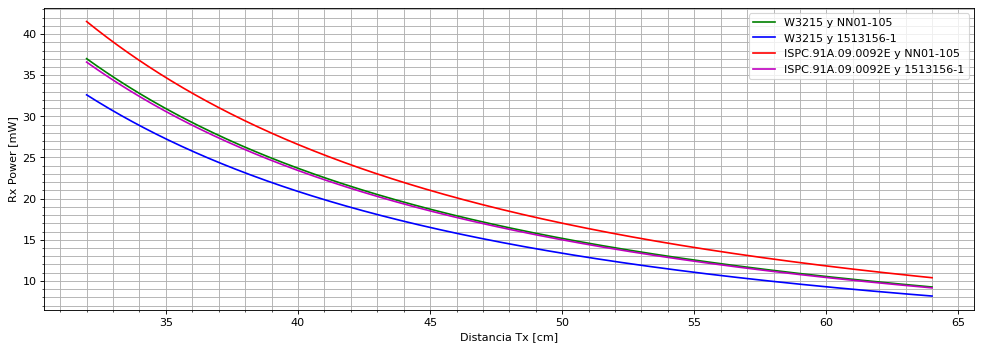
\includegraphics[width=\linewidth]{ImagenesFactibilidad/pot_recibida_teorica}
	\label{fig:pot_recibida_teorica}
	\caption{Potencia recibida en la antena Rx en función de la distancia entre antena Tx y antena Rx.}
\end{figure}

Se puede observar que con $4 \ W$ en la antena transmisora, todas las combinaciones de antenas cumplen con la potencia necesaria para el mejor y peor caso. Tomando el mejor par Rx-Tx, y al tener en cuenta la eficiencia de aproximadamente $70\%$ del P1110, la potencia a la salida de este permanece por encima del peor caso hasta la máxima distancia de transmisión.

\begin{figure}[H]
	\centering
	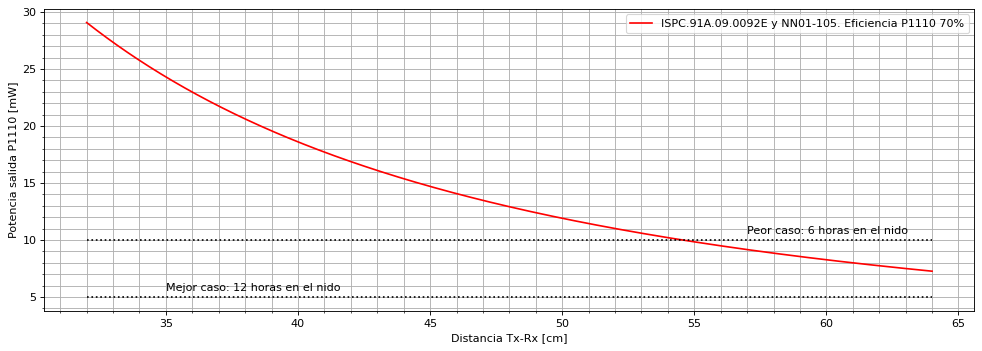
\includegraphics[width=\linewidth]{ImagenesFactibilidad/pot_baterias_teorica}
	\label{fig:pot_baterias_teorica}
	\caption{Potencia a la salida del P1110 en función de la distancia entre antena Tx y antena Rx.}
\end{figure}

Sin embargo, si se toma en consideración la restricción más estricta de $4.5 \  \frac{W}{m^2}$ impuesta en la Sección (\ref{sec:legal}) dada por la fórmula

\begin{equation}
	p = \frac{P_TG_T}{4\pi R^2}
\end{equation}

se observa en la Figura (\ref{fig:densidadradiada}) que para una potencia de $1.6 \ W$ en la antena transmisora esta restricción se cumple a treinta centímetros de la distancia mínima de transmisión.

\observacion{\verObs}{actualizar foto}
\begin{figure}[H]
	\centering
	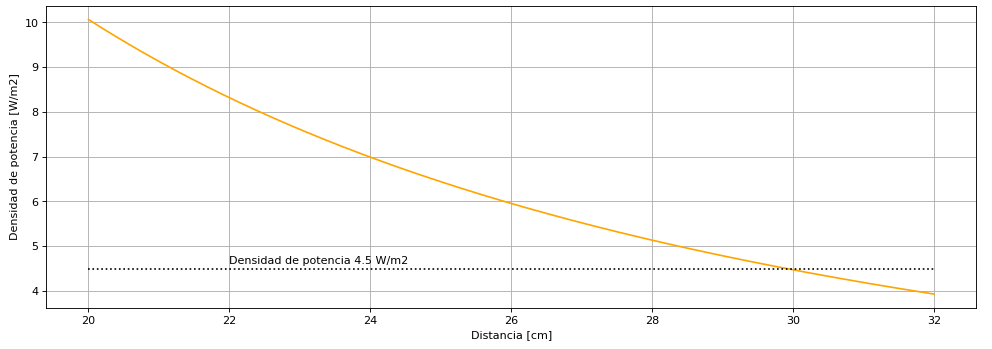
\includegraphics[width=\linewidth]{ImagenesFactibilidad/densidadradiada}
	\caption{Densidad de potencia radiada con $1.6 \ W$ en la antena transmisora según la fórmula de Friis.}
	\label{fig:densidadradiada}
\end{figure}

Teniendo esto en cuenta, y recalculando para $1.6 \ W$ se obtiene

\begin{figure}[H]
	\centering
	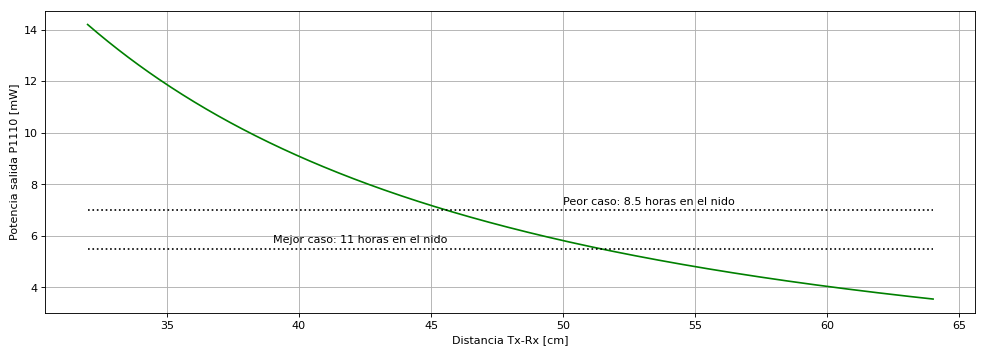
\includegraphics[width=\linewidth]{ImagenesFactibilidad/recalculo}
	\caption{Potencia a la salida del P1110 en función de la distancia entre antena Tx y antena Rx para $1.6 \ W$ en la antena transmisora.}
	\label{fig:recalculo}
\end{figure}

Por estas razones, se deberá complementar la recarga de la UBM utilizando un panel solar.


\Subsubsection{DFMEA}
\begin{adjustbox}{angle=90, captionbelow={DFMEA (Parte 1).}, float={table}[H]}

%CAMBIAR TODOS LOS CCC POR CCCCCC
\setlength\arrayrulewidth{0.5pt}
\centering
\begin{tabular}{|ccccccccccccc|}
\hline
\multicolumn{13}{|c|}{ANÁLISIS DE RIESGOS}                                                                                                                                                                                                                                                                                                                                                                                                                                                                                                                                                                                                                                                                                                                                                                                                                                                                                                                                                                                                                                             \\
\multicolumn{1}{|l}{}                                              & \multicolumn{1}{l}{}                                                                                                      & \multicolumn{1}{l}{}                                                                                                      & \multicolumn{1}{l}{}                                                                                                                                    & \multicolumn{1}{l}{}                            & \multicolumn{1}{l}{}                            & \multicolumn{1}{l}{}                            & \multicolumn{1}{l}{}                            & \multicolumn{1}{l}{}                                                                                                                                                                                 & \multicolumn{1}{l}{}                            & \multicolumn{1}{l}{}                            & \multicolumn{1}{l}{}                            & \multicolumn{1}{l|}{}      \\ \cline{2-8}
\multicolumn{1}{|l|}{}                                             & \multicolumn{1}{c|}{\begin{tabular}[c]{@{}c@{}}Fecha de\\ elaboración:\end{tabular}}                                      & \multicolumn{1}{c|}{25/05/21}                                                                                             & \multicolumn{1}{c|}{\begin{tabular}[c]{@{}c@{}}Fecha de\\ revisión:\end{tabular}}                                                                       & \multicolumn{4}{c|}{01/10/22}                                                                                                                                                                         & \multicolumn{1}{l}{}                                                                                                                                                                                 & \multicolumn{1}{l}{}                            & \multicolumn{1}{l}{}                            & \multicolumn{1}{l}{}                            & \multicolumn{1}{l|}{}      \\ \cline{2-8}
\multicolumn{1}{|l}{}                                              & \multicolumn{1}{l}{}                                                                                                      & \multicolumn{1}{l}{}                                                                                                      & \multicolumn{1}{l}{}                                                                                                                                    & \multicolumn{1}{l}{}                            & \multicolumn{1}{l}{}                            & \multicolumn{1}{l}{}                            & \multicolumn{1}{l}{}                            & \multicolumn{1}{l}{}                                                                                                                                                                                 & \multicolumn{1}{l}{}                            & \multicolumn{1}{l}{}                            & \multicolumn{1}{l}{}                            & \multicolumn{1}{l|}{}      \\ \hline
\rowcolor[HTML]{CCCCCC} 
\multicolumn{1}{|c|}{\cellcolor[HTML]{CCCCCC}}                     & \multicolumn{1}{c|}{\cellcolor[HTML]{CCCCCC}}                                                                             & \multicolumn{1}{c|}{\cellcolor[HTML]{CCCCCC}}                                                                             & \multicolumn{1}{c|}{\cellcolor[HTML]{CCCCCC}}                                                                                                           & \multicolumn{4}{c|}{\cellcolor[HTML]{CCCCCC}Aceptabilidad}                                                                                                                                            & \multicolumn{1}{c|}{\cellcolor[HTML]{CCCCCC}}                                                                                                                                                        & \multicolumn{4}{c|}{\cellcolor[HTML]{CCCCCC}Aceptabilidad}                                                                                                                       \\ \cline{5-8} \cline{10-13} 
\rowcolor[HTML]{CCCCCC} 
\multicolumn{1}{|c|}{\multirow{-2}{*}{\cellcolor[HTML]{CCCCCC}N°}} & \multicolumn{1}{c|}{\multirow{-2}{*}{\cellcolor[HTML]{CCCCCC}\begin{tabular}[c]{@{}c@{}}Efectos de\\ falla\end{tabular}}} & \multicolumn{1}{c|}{\multirow{-2}{*}{\cellcolor[HTML]{CCCCCC}\begin{tabular}[c]{@{}c@{}}Modo de\\ la falla\end{tabular}}} & \multicolumn{1}{c|}{\multirow{-2}{*}{\cellcolor[HTML]{CCCCCC}\begin{tabular}[c]{@{}c@{}}Causas de\\ la falla\end{tabular}}}                             & \multicolumn{1}{c|}{\cellcolor[HTML]{CCCCCC}NS} & \multicolumn{1}{c|}{\cellcolor[HTML]{CCCCCC}PO} & \multicolumn{1}{c|}{\cellcolor[HTML]{CCCCCC}DE} & \multicolumn{1}{c|}{\cellcolor[HTML]{CCCCCC}IC} & \multicolumn{1}{c|}{\multirow{-2}{*}{\cellcolor[HTML]{CCCCCC}\begin{tabular}[c]{@{}c@{}}Acción de\\ reducción\end{tabular}}}                                                                         & \multicolumn{1}{c|}{\cellcolor[HTML]{CCCCCC}NS} & \multicolumn{1}{c|}{\cellcolor[HTML]{CCCCCC}PO} & \multicolumn{1}{c|}{\cellcolor[HTML]{CCCCCC}DE} & IC                         \\ \hline
\multicolumn{1}{|c|}{1}                                            & \multicolumn{1}{c|}{\begin{tabular}[c]{@{}c@{}}No se pueden\\ realizar mediciones\end{tabular}}                           & \multicolumn{1}{c|}{\begin{tabular}[c]{@{}c@{}}Los sensores dejan\\ de funcionar\end{tabular}}                            & \multicolumn{1}{c|}{\begin{tabular}[c]{@{}c@{}}Los sensores\\ son dañados\\ por el ave\end{tabular}}                                                    & \multicolumn{1}{c|}{4}                          & \multicolumn{1}{c|}{4}                          & \multicolumn{1}{c|}{2}                          & \multicolumn{1}{c|}{\cellcolor[HTML]{F1C232}32} & \multicolumn{1}{c|}{\begin{tabular}[c]{@{}c@{}}Ocultar los sensores\\ en la bóveda\end{tabular}}                                                                                                     & \multicolumn{1}{c|}{4}                          & \multicolumn{1}{c|}{2}                          & \multicolumn{1}{c|}{2}                          & \cellcolor[HTML]{6AA84F}16 \\ \hline
\multicolumn{1}{|c|}{2}                                            & \multicolumn{1}{c|}{\begin{tabular}[c]{@{}c@{}}No se pueden\\ realizar mediciones\end{tabular}}                           & \multicolumn{1}{c|}{\begin{tabular}[c]{@{}c@{}}Los sensores dejan\\ de funcionar\end{tabular}}                            & \multicolumn{1}{c|}{\begin{tabular}[c]{@{}c@{}}El conexionado es\\ dañado por el ave\end{tabular}}                                                      & \multicolumn{1}{c|}{4}                          & \multicolumn{1}{c|}{4}                          & \multicolumn{1}{c|}{2}                          & \multicolumn{1}{c|}{\cellcolor[HTML]{F1C232}32} & \multicolumn{1}{c|}{\begin{tabular}[c]{@{}c@{}}Hacer más\\ robusto el cableado\end{tabular}}                                                                                                         & \multicolumn{1}{c|}{4}                          & \multicolumn{1}{c|}{2}                          & \multicolumn{1}{c|}{2}                          & \cellcolor[HTML]{6AA84F}16 \\ \hline
\multicolumn{1}{|c|}{3}                                            & \multicolumn{1}{c|}{Falta de energía solar}                                                                               & \multicolumn{1}{c|}{\begin{tabular}[c]{@{}c@{}}Falla en los\\ paneles solares\end{tabular}}                               & \multicolumn{1}{c|}{\begin{tabular}[c]{@{}c@{}}Los paneles se\\ encuentran dañados\end{tabular}}                                                        & \multicolumn{1}{c|}{5}                          & \multicolumn{1}{c|}{3}                          & \multicolumn{1}{c|}{2}                          & \multicolumn{1}{c|}{\cellcolor[HTML]{F1C232}30} & \multicolumn{1}{c|}{\begin{tabular}[c]{@{}c@{}}Colocar protección\\ para los paneles\end{tabular}}                                                                                                   & \multicolumn{1}{c|}{5}                          & \multicolumn{1}{c|}{2}                          & \multicolumn{1}{c|}{2}                          & \cellcolor[HTML]{6AA84F}20 \\ \hline
\multicolumn{1}{|c|}{4}                                            & \multicolumn{1}{c|}{Falta de energía solar}                                                                               & \multicolumn{1}{c|}{\begin{tabular}[c]{@{}c@{}}La electrónica no\\ funciona correctamente\end{tabular}}                   & \multicolumn{1}{c|}{\begin{tabular}[c]{@{}c@{}}Fue colocado en un\\ lugar con obstrucciones\end{tabular}}                                               & \multicolumn{1}{c|}{5}                          & \multicolumn{1}{c|}{3}                          & \multicolumn{1}{c|}{3}                          & \multicolumn{1}{c|}{\cellcolor[HTML]{F1C232}45} & \multicolumn{1}{c|}{\begin{tabular}[c]{@{}c@{}}Instalar el panel solar\\ sobre un tronco,\\ donde no haya ramas\\ u objetos que\\ puedan obstruir\end{tabular}}                                        & \multicolumn{1}{c|}{5}                          & \multicolumn{1}{c|}{1}                          & \multicolumn{1}{c|}{3}                          & \cellcolor[HTML]{6AA84F}15 \\ \hline
\multicolumn{1}{|c|}{5}                                            & \multicolumn{1}{c|}{\begin{tabular}[c]{@{}c@{}}Falta de energía\\ en la UBN\end{tabular}}                                 & \multicolumn{1}{c|}{No hay alimentación}                                                                                  & \multicolumn{1}{c|}{\begin{tabular}[c]{@{}c@{}}\TBD días con un nivel\\ de luz menor al necesario\\ para la carga de baterías\end{tabular}}             & \multicolumn{1}{c|}{5}                          & \multicolumn{1}{c|}{3}                          & \multicolumn{1}{c|}{3}                          & \multicolumn{1}{c|}{\cellcolor[HTML]{F1C232}45} & \multicolumn{1}{c|}{\begin{tabular}[c]{@{}c@{}}Seleccionar una\\ batería más grande\\ de la necesaria\\ para almacenar\\ un excedente\end{tabular}}                                                    & \multicolumn{1}{c|}{5}                          & \multicolumn{1}{c|}{1}                          & \multicolumn{1}{c|}{3}                          & \cellcolor[HTML]{6AA84F}15 \\ \hline
\multicolumn{1}{|c|}{6}                                            & \multicolumn{1}{c|}{\begin{tabular}[c]{@{}c@{}}Falta de energía\\ en la UBN\end{tabular}}                                 & \multicolumn{1}{c|}{La batería no funciona}                                                                               & \multicolumn{1}{c|}{\begin{tabular}[c]{@{}c@{}}Se inundó el contenedor\\ de la batería\end{tabular}}                                                    & \multicolumn{1}{c|}{5}                          & \multicolumn{1}{c|}{3}                          & \multicolumn{1}{c|}{4}                          & \multicolumn{1}{c|}{\cellcolor[HTML]{CC0000}60} & \multicolumn{1}{c|}{\begin{tabular}[c]{@{}c@{}}Se utiliza una carcasa\\ para la batería con\\ protección \TBD que\\ asegure protección\\ contra agua\end{tabular}}                                   & \multicolumn{1}{c|}{5}                          & \multicolumn{1}{c|}{1}                          & \multicolumn{1}{c|}{4}                          & \cellcolor[HTML]{6AA84F}20 \\ \hline
\end{tabular}

\end{adjustbox}

\newpage

\begin{adjustbox}{angle=90, captionbelow={DFMEA (Parte 2).}, float={table}[H]}

%CAMBIAR TODOS LOS CCC POR CCCCCC
\setlength\arrayrulewidth{0.5pt}
\centering
\begin{tabular}{|ccccccccccccc|}
\hline
\multicolumn{13}{|c|}{ANÁLISIS DE RIESGOS}                                                                                                                                                                                                                                                                                                                                                                                                                                                                                                                                                                                                                                                                                                                                                                                                                                                                                                                                                                                                                                             \\
\multicolumn{1}{|l}{}                                              & \multicolumn{1}{l}{}                                                                                                      & \multicolumn{1}{l}{}                                                                                                      & \multicolumn{1}{l}{}                                                                                                                                    & \multicolumn{1}{l}{}                            & \multicolumn{1}{l}{}                            & \multicolumn{1}{l}{}                            & \multicolumn{1}{l}{}                            & \multicolumn{1}{l}{}                                                                                                                                                                                 & \multicolumn{1}{l}{}                            & \multicolumn{1}{l}{}                            & \multicolumn{1}{l}{}                            & \multicolumn{1}{l|}{}      \\ \cline{2-8}
\multicolumn{1}{|l|}{}                                             & \multicolumn{1}{c|}{\begin{tabular}[c]{@{}c@{}}Fecha de\\ elaboración:\end{tabular}}                                      & \multicolumn{1}{c|}{25/05/21}                                                                                             & \multicolumn{1}{c|}{\begin{tabular}[c]{@{}c@{}}Fecha de\\ revisión:\end{tabular}}                                                                       & \multicolumn{4}{c|}{01/10/22}                                                                                                                                                                         & \multicolumn{1}{l}{}                                                                                                                                                                                 & \multicolumn{1}{l}{}                            & \multicolumn{1}{l}{}                            & \multicolumn{1}{l}{}                            & \multicolumn{1}{l|}{}      \\ \cline{2-8}
\multicolumn{1}{|l}{}                                              & \multicolumn{1}{l}{}                                                                                                      & \multicolumn{1}{l}{}                                                                                                      & \multicolumn{1}{l}{}                                                                                                                                    & \multicolumn{1}{l}{}                            & \multicolumn{1}{l}{}                            & \multicolumn{1}{l}{}                            & \multicolumn{1}{l}{}                            & \multicolumn{1}{l}{}                                                                                                                                                                                 & \multicolumn{1}{l}{}                            & \multicolumn{1}{l}{}                            & \multicolumn{1}{l}{}                            & \multicolumn{1}{l|}{}      \\ \hline
\rowcolor[HTML]{CCCCCC} 
\multicolumn{1}{|c|}{\cellcolor[HTML]{CCCCCC}}                     & \multicolumn{1}{c|}{\cellcolor[HTML]{CCCCCC}}                                                                             & \multicolumn{1}{c|}{\cellcolor[HTML]{CCCCCC}}                                                                             & \multicolumn{1}{c|}{\cellcolor[HTML]{CCCCCC}}                                                                                                           & \multicolumn{4}{c|}{\cellcolor[HTML]{CCCCCC}Aceptabilidad}                                                                                                                                            & \multicolumn{1}{c|}{\cellcolor[HTML]{CCCCCC}}                                                                                                                                                        & \multicolumn{4}{c|}{\cellcolor[HTML]{CCCCCC}Aceptabilidad}                                                                                                                       \\ \cline{5-8} \cline{10-13} 
\rowcolor[HTML]{CCCCCC} 
\multicolumn{1}{|c|}{\multirow{-2}{*}{\cellcolor[HTML]{CCCCCC}N°}} & \multicolumn{1}{c|}{\multirow{-2}{*}{\cellcolor[HTML]{CCCCCC}\begin{tabular}[c]{@{}c@{}}Efectos de\\ falla\end{tabular}}} & \multicolumn{1}{c|}{\multirow{-2}{*}{\cellcolor[HTML]{CCCCCC}\begin{tabular}[c]{@{}c@{}}Modo de\\ la falla\end{tabular}}} & \multicolumn{1}{c|}{\multirow{-2}{*}{\cellcolor[HTML]{CCCCCC}\begin{tabular}[c]{@{}c@{}}Causas de\\ la falla\end{tabular}}}                             & \multicolumn{1}{c|}{\cellcolor[HTML]{CCCCCC}NS} & \multicolumn{1}{c|}{\cellcolor[HTML]{CCCCCC}PO} & \multicolumn{1}{c|}{\cellcolor[HTML]{CCCCCC}DE} & \multicolumn{1}{c|}{\cellcolor[HTML]{CCCCCC}IC} & \multicolumn{1}{c|}{\multirow{-2}{*}{\cellcolor[HTML]{CCCCCC}\begin{tabular}[c]{@{}c@{}}Acción de\\ reducción\end{tabular}}}                                                                         & \multicolumn{1}{c|}{\cellcolor[HTML]{CCCCCC}NS} & \multicolumn{1}{c|}{\cellcolor[HTML]{CCCCCC}PO} & \multicolumn{1}{c|}{\cellcolor[HTML]{CCCCCC}DE} & IC                         \\ \hline
\multicolumn{1}{|c|}{7}                                            & \multicolumn{1}{c|}{\begin{tabular}[c]{@{}c@{}}La electrónica\\ deja de funcionar\end{tabular}}                                        & \multicolumn{1}{c|}{\begin{tabular}[c]{@{}c@{}}La UP deja\\ de funcionar\end{tabular}}                                            & \multicolumn{1}{c|}{\begin{tabular}[c]{@{}c@{}}La UP se\\ encuentra a una\\ temperatura baja\end{tabular}}                                              & \multicolumn{1}{c|}{5}                          & \multicolumn{1}{c|}{2}                          & \multicolumn{1}{c|}{2}                          & \multicolumn{1}{c|}{\cellcolor[HTML]{6AA84F}20} & \multicolumn{1}{c|}{\begin{tabular}[c]{@{}c@{}}Colocar la UP en\\ un encapsulado\end{tabular}}                                                                                                       & \multicolumn{1}{c|}{5}                          & \multicolumn{1}{c|}{1}                          & \multicolumn{1}{c|}{2}                          & \cellcolor[HTML]{6AA84F}10 \\ \hline
\multicolumn{1}{|c|}{8}                                            & \multicolumn{1}{c|}{\begin{tabular}[c]{@{}c@{}}Falla de\\ almacenamiento\end{tabular}}                                                 & \multicolumn{1}{c|}{\begin{tabular}[c]{@{}c@{}}No se pueden\\ guardar más datos\end{tabular}}                                     & \multicolumn{1}{c|}{\begin{tabular}[c]{@{}c@{}}La temperatura de\\ operación es menor\\ al mínimo aceptable\end{tabular}}                               & \multicolumn{1}{c|}{5}                          & \multicolumn{1}{c|}{4}                          & \multicolumn{1}{c|}{3}                          & \multicolumn{1}{c|}{\cellcolor[HTML]{CC0000}60} & \multicolumn{1}{c|}{\begin{tabular}[c]{@{}c@{}}Cambiar la\\ memoria por una de\\ nivel industrial\end{tabular}}                                                                                      & \multicolumn{1}{c|}{5}                          & \multicolumn{1}{c|}{1}                          & \multicolumn{1}{c|}{3}                          & \cellcolor[HTML]{6AA84F}15 \\ \hline
\multicolumn{1}{|c|}{9}                                            & \multicolumn{1}{c|}{\begin{tabular}[c]{@{}c@{}}Falla de\\ almacenamiento\end{tabular}}                                                 & \multicolumn{1}{c|}{\begin{tabular}[c]{@{}c@{}}La memoria sufre una\\ pérdida de información\end{tabular}}                        & \multicolumn{1}{c|}{\begin{tabular}[c]{@{}c@{}}La memoria\\ es defectuosa\end{tabular}}                                                                 & \multicolumn{1}{c|}{5}                          & \multicolumn{1}{c|}{2}                          & \multicolumn{1}{c|}{3}                          & \multicolumn{1}{c|}{\cellcolor[HTML]{F1C232}30} & \multicolumn{1}{c|}{\begin{tabular}[c]{@{}c@{}}Se verifica la\\ funcionaldad de la\\ misma antes de\\ integrarla al proyecto\end{tabular}}                                                           & \multicolumn{1}{c|}{5}                          & \multicolumn{1}{c|}{1}                          & \multicolumn{1}{c|}{3}                          & \cellcolor[HTML]{6AA84F}15 \\ \hline
\multicolumn{1}{|c|}{10}                                           & \multicolumn{1}{c|}{\begin{tabular}[c]{@{}c@{}}Interrupción en\\ la transmisión\\ nido - base principal\\ de seguimiento\end{tabular}} & \multicolumn{1}{c|}{\begin{tabular}[c]{@{}c@{}}Se pierde la\\ comunicación\\ con la base principal\\ de seguimiento\end{tabular}} & \multicolumn{1}{c|}{\begin{tabular}[c]{@{}c@{}}La base principal\\ de seguimiento es\\ colocada fuera del rango\\ de la comunicación\end{tabular}}      & \multicolumn{1}{c|}{5}                          & \multicolumn{1}{c|}{3}                          & \multicolumn{1}{c|}{2}                          & \multicolumn{1}{c|}{\cellcolor[HTML]{F1C232}30} & \multicolumn{1}{c|}{\begin{tabular}[c]{@{}c@{}}Se verifica el alcance\\ de la transmisión de la base\\ principal de seguimiento\\ luego de su colocación\end{tabular}}                               & \multicolumn{1}{c|}{5}                          & \multicolumn{1}{c|}{1}                          & \multicolumn{1}{c|}{2}                          & \cellcolor[HTML]{6AA84F}10 \\ \hline
\multicolumn{1}{|c|}{11}                                           & \multicolumn{1}{c|}{\begin{tabular}[c]{@{}c@{}}Interrupción en\\ la transmisión\\ nido - persona\end{tabular}}                         & \multicolumn{1}{c|}{\begin{tabular}[c]{@{}c@{}}Se pierde la\\ comunicación\\ con la persona\end{tabular}}                         & \multicolumn{1}{c|}{\begin{tabular}[c]{@{}c@{}}El dispositivo receptor\\ no se encuentra en\\ el rango de transmisión\end{tabular}}                     & \multicolumn{1}{c|}{5}                          & \multicolumn{1}{c|}{3}                          & \multicolumn{1}{c|}{2}                          & \multicolumn{1}{c|}{\cellcolor[HTML]{F1C232}30} & \multicolumn{1}{c|}{\begin{tabular}[c]{@{}c@{}}Informar la existencia\\ del error en el\\ dispositivo receptor\end{tabular}}                                                                         & \multicolumn{1}{c|}{3}                          & \multicolumn{1}{c|}{3}                          & \multicolumn{1}{c|}{2}                          & \cellcolor[HTML]{6AA84F}18 \\ \hline
\multicolumn{1}{|c|}{12}                                           & \multicolumn{1}{c|}{\begin{tabular}[c]{@{}c@{}}Interrupción en\\ la transmisión\\ nido - persona\end{tabular}}                         & \multicolumn{1}{c|}{\begin{tabular}[c]{@{}c@{}}La transmisión de datos\\ se ve interrumpida\end{tabular}}                         & \multicolumn{1}{c|}{\begin{tabular}[c]{@{}c@{}}La persona que recibe la\\ información está\\ posicionada demasiado\\ lejos del transmisor\end{tabular}} & \multicolumn{1}{c|}{4}                          & \multicolumn{1}{c|}{2}                          & \multicolumn{1}{c|}{2}                          & \multicolumn{1}{c|}{\cellcolor[HTML]{6AA84F}16} & \multicolumn{1}{c|}{\begin{tabular}[c]{@{}c@{}}La información es\\ borrada únicamente\\ cuando se recibe\\ un mensaje de OK\\ de la persona en la\\ base del árbol\\ a través del WIFI\end{tabular}} & \multicolumn{1}{c|}{2}                          & \multicolumn{1}{c|}{2}                          & \multicolumn{1}{c|}{2}                          & \cellcolor[HTML]{6AA84F}8  \\ \hline
\end{tabular}

\end{adjustbox}

\newpage

\begin{adjustbox}{angle=90, captionbelow={DFMEA (Parte 3).}, float={table}[H]}

%CAMBIAR TODOS LOS CCC POR CCCCCC
\setlength\arrayrulewidth{0.5pt}
\centering
\begin{tabular}{|ccccccccccccc|}
\hline
\multicolumn{13}{|c|}{ANÁLISIS DE RIESGOS}                                                                                                                                                                                                                                                                                                                                                                                                                                                                                                                                                                                                                                                                                                                                                                                                                                                                                                                                                                                           \\
\multicolumn{1}{|l}{}                                              & \multicolumn{1}{l}{}                                                                                                      & \multicolumn{1}{l}{}                                                                                                      & \multicolumn{1}{l}{}                                                                                                        & \multicolumn{1}{l}{}                            & \multicolumn{1}{l}{}                            & \multicolumn{1}{l}{}                            & \multicolumn{1}{l}{}                            & \multicolumn{1}{l}{}                                                                                                                                                           & \multicolumn{1}{l}{}                            & \multicolumn{1}{l}{}                            & \multicolumn{1}{l}{}                            & \multicolumn{1}{l|}{}      \\ \cline{2-8}
\multicolumn{1}{|l|}{}                                             & \multicolumn{1}{c|}{\begin{tabular}[c]{@{}c@{}}Fecha de\\ elaboración:\end{tabular}}                                      & \multicolumn{1}{c|}{25/05/21}                                                                                             & \multicolumn{1}{c|}{\begin{tabular}[c]{@{}c@{}}Fecha de\\ revisión:\end{tabular}}                                           & \multicolumn{4}{c|}{01/10/22}                                                                                                                                                                         & \multicolumn{1}{l}{}                                                                                                                                                           & \multicolumn{1}{l}{}                            & \multicolumn{1}{l}{}                            & \multicolumn{1}{l}{}                            & \multicolumn{1}{l|}{}      \\ \cline{2-8}
\multicolumn{1}{|l}{}                                              & \multicolumn{1}{l}{}                                                                                                      & \multicolumn{1}{l}{}                                                                                                      & \multicolumn{1}{l}{}                                                                                                        & \multicolumn{1}{l}{}                            & \multicolumn{1}{l}{}                            & \multicolumn{1}{l}{}                            & \multicolumn{1}{l}{}                            & \multicolumn{1}{l}{}                                                                                                                                                           & \multicolumn{1}{l}{}                            & \multicolumn{1}{l}{}                            & \multicolumn{1}{l}{}                            & \multicolumn{1}{l|}{}      \\ \hline
\rowcolor[HTML]{CCCCCC} 
\multicolumn{1}{|c|}{\cellcolor[HTML]{CCCCCC}}                     & \multicolumn{1}{c|}{\cellcolor[HTML]{CCCCCC}}                                                                             & \multicolumn{1}{c|}{\cellcolor[HTML]{CCCCCC}}                                                                             & \multicolumn{1}{c|}{\cellcolor[HTML]{CCCCCC}}                                                                               & \multicolumn{4}{c|}{\cellcolor[HTML]{CCCCCC}Aceptabilidad}                                                                                                                                            & \multicolumn{1}{c|}{\cellcolor[HTML]{CCCCCC}}                                                                                                                                  & \multicolumn{4}{c|}{\cellcolor[HTML]{CCCCCC}Aceptabilidad}                                                                                                                       \\ \cline{5-8} \cline{10-13} 
\rowcolor[HTML]{CCCCCC} 
\multicolumn{1}{|c|}{\multirow{-2}{*}{\cellcolor[HTML]{CCCCCC}N°}} & \multicolumn{1}{c|}{\multirow{-2}{*}{\cellcolor[HTML]{CCCCCC}\begin{tabular}[c]{@{}c@{}}Efectos de\\ falla\end{tabular}}} & \multicolumn{1}{c|}{\multirow{-2}{*}{\cellcolor[HTML]{CCCCCC}\begin{tabular}[c]{@{}c@{}}Modo de\\ la falla\end{tabular}}} & \multicolumn{1}{c|}{\multirow{-2}{*}{\cellcolor[HTML]{CCCCCC}\begin{tabular}[c]{@{}c@{}}Causas de\\ la falla\end{tabular}}} & \multicolumn{1}{c|}{\cellcolor[HTML]{CCCCCC}NS} & \multicolumn{1}{c|}{\cellcolor[HTML]{CCCCCC}PO} & \multicolumn{1}{c|}{\cellcolor[HTML]{CCCCCC}DE} & \multicolumn{1}{c|}{\cellcolor[HTML]{CCCCCC}IC} & \multicolumn{1}{c|}{\multirow{-2}{*}{\cellcolor[HTML]{CCCCCC}\begin{tabular}[c]{@{}c@{}}Acción de\\ reducción\end{tabular}}}                                                   & \multicolumn{1}{c|}{\cellcolor[HTML]{CCCCCC}NS} & \multicolumn{1}{c|}{\cellcolor[HTML]{CCCCCC}PO} & \multicolumn{1}{c|}{\cellcolor[HTML]{CCCCCC}DE} & IC                         \\ \hline
\multicolumn{1}{|c|}{13}                                           & \multicolumn{1}{c|}{\begin{tabular}[c]{@{}c@{}}No se detecta el ave\\ nunca en el nido\end{tabular}}                                   & \multicolumn{1}{c|}{\begin{tabular}[c]{@{}c@{}}Falla la detección del\\ ave en el nido\end{tabular}}                              & \multicolumn{1}{c|}{\begin{tabular}[c]{@{}c@{}}La \rpi no consigue\\ detectar la señal del\\ beacon del ave fuera\\ del nido\end{tabular}}              & \multicolumn{1}{c|}{5}                          & \multicolumn{1}{c|}{4}                          & \multicolumn{1}{c|}{3}                          & \multicolumn{1}{c|}{\cellcolor[HTML]{CC0000}60} & \multicolumn{1}{c|}{\begin{tabular}[c]{@{}c@{}}Se realiza la detección\\ del ave utilizando\\ un módulo BLE en\\ la placa de sensores\\ dentro del nido\end{tabular}}                                & \multicolumn{1}{c|}{5}                          & \multicolumn{1}{c|}{1}                          & \multicolumn{1}{c|}{3}                          & \cellcolor[HTML]{6AA84F}15 \\ \hline
\multicolumn{1}{|c|}{14}                                           & \multicolumn{1}{c|}{Falla en el servidor}                                                                                              & \multicolumn{1}{c|}{\begin{tabular}[c]{@{}c@{}}No se obtiene\\ respuesta\\ de \nodered\end{tabular}}                              & \multicolumn{1}{c|}{Sobrecarga del servidor}                                                                                                            & \multicolumn{1}{c|}{4}                          & \multicolumn{1}{c|}{3}                          & \multicolumn{1}{c|}{5}                          & \multicolumn{1}{c|}{\cellcolor[HTML]{CC0000}60} & \multicolumn{1}{c|}{\begin{tabular}[c]{@{}c@{}}Reiniciar \nodered cada\\ cierto tiempo así se\\ refresca el servidor\end{tabular}}                                                                   & \multicolumn{1}{c|}{4}                          & \multicolumn{1}{c|}{1}                          & \multicolumn{1}{c|}{5}                          & \cellcolor[HTML]{6AA84F}20 \\ \hline
\multicolumn{1}{|c|}{15}                                           & \multicolumn{1}{c|}{Falla en el servidor}                                                                                              & \multicolumn{1}{c|}{\begin{tabular}[c]{@{}c@{}}No se obtiene\\ respuesta\\ de \nodered\end{tabular}}                              & \multicolumn{1}{c|}{\begin{tabular}[c]{@{}c@{}}Reiteradas solicitudes\\ el usuario de un mismo\\ servicio\end{tabular}}                                 & \multicolumn{1}{c|}{5}                          & \multicolumn{1}{c|}{5}                          & \multicolumn{1}{c|}{1}                          & \multicolumn{1}{c|}{\cellcolor[HTML]{6AA84F}25} & \multicolumn{1}{c|}{\begin{tabular}[c]{@{}c@{}}Identificar si ya se solicitó el\\ servicio y bloquear el\\ ingreso de solicitudes\end{tabular}}                                                      & \multicolumn{1}{c|}{5}                          & \multicolumn{1}{c|}{1}                          & \multicolumn{1}{c|}{1}                          & \cellcolor[HTML]{6AA84F}5  \\ \hline
\multicolumn{1}{|c|}{16}                                           & \multicolumn{1}{c|}{Falla en el servidor}                                                                                              & \multicolumn{1}{c|}{\begin{tabular}[c]{@{}c@{}}No se puede visualizar\\ el nido en tiempo real\end{tabular}}                      & \multicolumn{1}{c|}{\begin{tabular}[c]{@{}c@{}}Sobrecarga debido a una\\ transmisión sonstante\end{tabular}}                                            & \multicolumn{1}{c|}{5}                          & \multicolumn{1}{c|}{5}                          & \multicolumn{1}{c|}{3}                          & \multicolumn{1}{c|}{\cellcolor[HTML]{CC0000}75} & \multicolumn{1}{c|}{\begin{tabular}[c]{@{}c@{}}Limitar el tiempo de\\ transmisión a un período de\\ 5 minutos y brindar la\\ posibilidad de reiniciar el\\ video\end{tabular}}                       & \multicolumn{1}{c|}{5}                          & \multicolumn{1}{c|}{1}                          & \multicolumn{1}{c|}{3}                          & \cellcolor[HTML]{6AA84F}15 \\ \hline
\multicolumn{1}{|c|}{17}                                           & \multicolumn{1}{c|}{\begin{tabular}[c]{@{}c@{}}Inconsistencia del\\ intervalo de tiempo\\ entre mediciones\end{tabular}}               & \multicolumn{1}{c|}{\begin{tabular}[c]{@{}c@{}}Se pierde seguimiento\\ del último dato tomado\end{tabular}}                       & \multicolumn{1}{c|}{\begin{tabular}[c]{@{}c@{}}Se sobrecarga\\ temporalmente o se\\ reinicia el servidor\end{tabular}}                                  & \multicolumn{1}{c|}{4}                          & \multicolumn{1}{c|}{4}                          & \multicolumn{1}{c|}{2}                          & \multicolumn{1}{c|}{\cellcolor[HTML]{F1C232}32} & \multicolumn{1}{c|}{\begin{tabular}[c]{@{}c@{}}Se almacena en memoria la\\ fecha y hora de la última\\ medición\end{tabular}}                                                                        & \multicolumn{1}{c|}{4}                          & \multicolumn{1}{c|}{1}                          & \multicolumn{1}{c|}{2}                          & \cellcolor[HTML]{6AA84F}8  \\ \hline

\end{tabular}

\end{adjustbox}

\newpage

\begin{multicols}{2}
\begin{table}[H]
\centering
\begin{tabular}{|c|c|c|c}
\cline{1-3}
Severidad                                                   & Probabilidad	& Detectabilidad 	& \multicolumn{1}{l}{}   \\ \hline
Insignificante                                              & Remota      	& Completa       	& \multicolumn{1}{c|}{1} \\ \hline
\begin{tabular}[c]{@{}c@{}}Poco\\ significante\end{tabular} & Poco remota	& Mayor          	& \multicolumn{1}{c|}{2} \\ \hline
Moderado                                                    & Media       	& Moderada       	& \multicolumn{1}{c|}{3} \\ \hline
Grave                                                       & Alta        	& Pequeña        	& \multicolumn{1}{c|}{4} \\ \hline
Muy grave                                                   & Muy alta    	& Mínima         	& \multicolumn{1}{c|}{5} \\ \hline
\end{tabular}
\caption{Criterio de IC.}
\label{dfmea:CriterioIC}
\end{table}

\begin{table}[H]
\setlength\arrayrulewidth{0.5pt}
\centering
\begin{tabular}{|c|c|}
\hline
\multicolumn{2}{|c|}{Nivel de IC}                                                                                      \\ \hline
\cellcolor[HTML]{6AA84F}Aceptable                                                                       & IC $\leq$ 27 \\ \hline
\cellcolor[HTML]{F1C232}\begin{tabular}[c]{@{}c@{}}Bajar hasta\\ razonablemente\\ práctico\end{tabular} & 27 < IC < 48 \\ \hline
\cellcolor[HTML]{CC0000}No aceptable                                                                       & 48 $\leq$ IC \\ \hline
\end{tabular}
\caption{Nivel de IC.}
\label{dfmea:nievlIC}
\end{table}
\end{multicols}

\Subsection{Factibilidad de Tiempos}

\Subsubsection{Consideraciones}
Para el desarrollo de las siguientes secciones, se tiene en cuenta un equipo de trabajo de 4 personas, con días laborales de 8 horas. Además se consideran 15 días de vacaciones en la primera quincena de enero.

\Subsubsection{Planificación}
Se procede a presentar un cuadro con las tareas a realizar. En la siguiente tabla se observa el tiempo más probable, el optimista y el pesimista, para tener un análisis más real de la duración.

\begin{table}[H]
\centering
\begin{tabular}{|c|c|c|c|c|c|}
\hline
\textbf{N°} & \textbf{Nombre de tarea}                												& \textbf{\begin{tabular}[c]{@{}c@{}}Duración\\ Optimista\end{tabular}} & \textbf{\begin{tabular}[c]{@{}c@{}}Duración\\ Media\end{tabular}} & \textbf{\begin{tabular}[c]{@{}c@{}}Duración\\ Pesimista\end{tabular}} & \textbf{Predecesora} \\ \hline
1           & Detectar Necesidad                      												& 1                           & 3           	  & 4                           & -                                         \\ \hline
2           & Definir el alcance                      												& 2                           & 3                 & 4                           & 1                                         \\ \hline
3           & Antecedentes y Contexto                 												& 1                           & 2                 & 3                           & 1                                         \\ \hline
4           & Reuniones con cliente             	  												& 0.25                        & 0.25              & 0.25                        & 1                                         \\ \hline
5           & Definir objetivos de diseño             												& 1                           & 2                 & 5                           & 2, 3                                      \\ \hline
6           & Definir requerimientos                  												& 4                           & 5                 & 8                           & 4, 5                                      \\ \hline
7           & Definir Especificaciones                												& 3                           & 5                 & 8                           & 5                                         \\ \hline
8           & Planes de validación                    												& 3                           & 5                 & 8                           & 11                                        \\ \hline
9           & DFMEA 1° reunión                        												& 0.25                        & 0.25              & 0.25                        & 8                                         \\ \hline
10          & \begin{tabular}[c]{@{}c@{}}Investigación antenas\\ y radiopropagación\end{tabular} 	& 44                          & 45                & 54                          & 6, 7                                      \\ \hline
11          & \begin{tabular}[c]{@{}c@{}}Análisis de\\ factibilidad Tecnológica\end{tabular}    	& 40                          & 45                & 47                          & 6, 7                                      \\ \hline
12          & \begin{tabular}[c]{@{}c@{}}Análisis de\\ presupuesto y costos\end{tabular}        	& 4                           & 5                 & 9                           & 6, 7                                      \\ \hline
13          & \begin{tabular}[c]{@{}c@{}}Análisis de\\ factibilidad económica\end{tabular}      	& 3                           & 5                 & 8                           & 12                                        \\ \hline
14          & DFMEA 2° reunión                        												& 0.25                        & 0.25              & 0.25                        & 9, 11, 12                                 \\ \hline
15          & Cálculo y selección de HW               												& 12                          & 15                & 20                          & 11, 12, 13                                \\ \hline
16          & \begin{tabular}[c]{@{}c@{}}Diagrama de HW y\\ plan de implementación\end{tabular} 	& 14                          & 15                & 18                          & 15                                        \\ \hline
17          & DFMEA 3° reunión                        												& 0.25                        & 0.25              & 0.25                        & 15                                        \\ \hline
18          & \begin{tabular}[c]{@{}c@{}}Diagrama de SW y\\ plan de implementación\end{tabular} 	& 11                          & 15                & 19                          & 15                                        \\ \hline
19          & Integración a nivel módulos             												& 23                          & 25                & 27                          & 16, 18                                    \\ \hline
20          & Integración general                     												& 18                          & 20                & 21                          & 19                                        \\ \hline
21          & Integración Prototipo                   												& 9                           & 12                & 13                          & 20                                        \\ \hline
22          & Vacaciones                              												& 15                          & 15                & 15                          & 21                                        \\ \hline
23          & Integración a Prototipo                 												& 9                           & 12                & 13                          & 22                                        \\ \hline
24          & Validación de prototipo                 												& 19                          & 20                & 21                          & 23                                        \\ \hline
25          & Estudio de confiabilidad                												& 6                           & 10                & 13                          & 24                                        \\ \hline
\end{tabular}
\caption{Actividades a realizar en el proyecto en días laborales de 8 horas cada uno.}
\label{tab:tareas}
\end{table}










\Subsubsection{Programación}
Se realizo un diagrama de Gantt acorde a la Tabla (\ref{tab:tareas}). En este se marcó el camino crítico en rojo.
\begin{figure}[H]
	\centering
	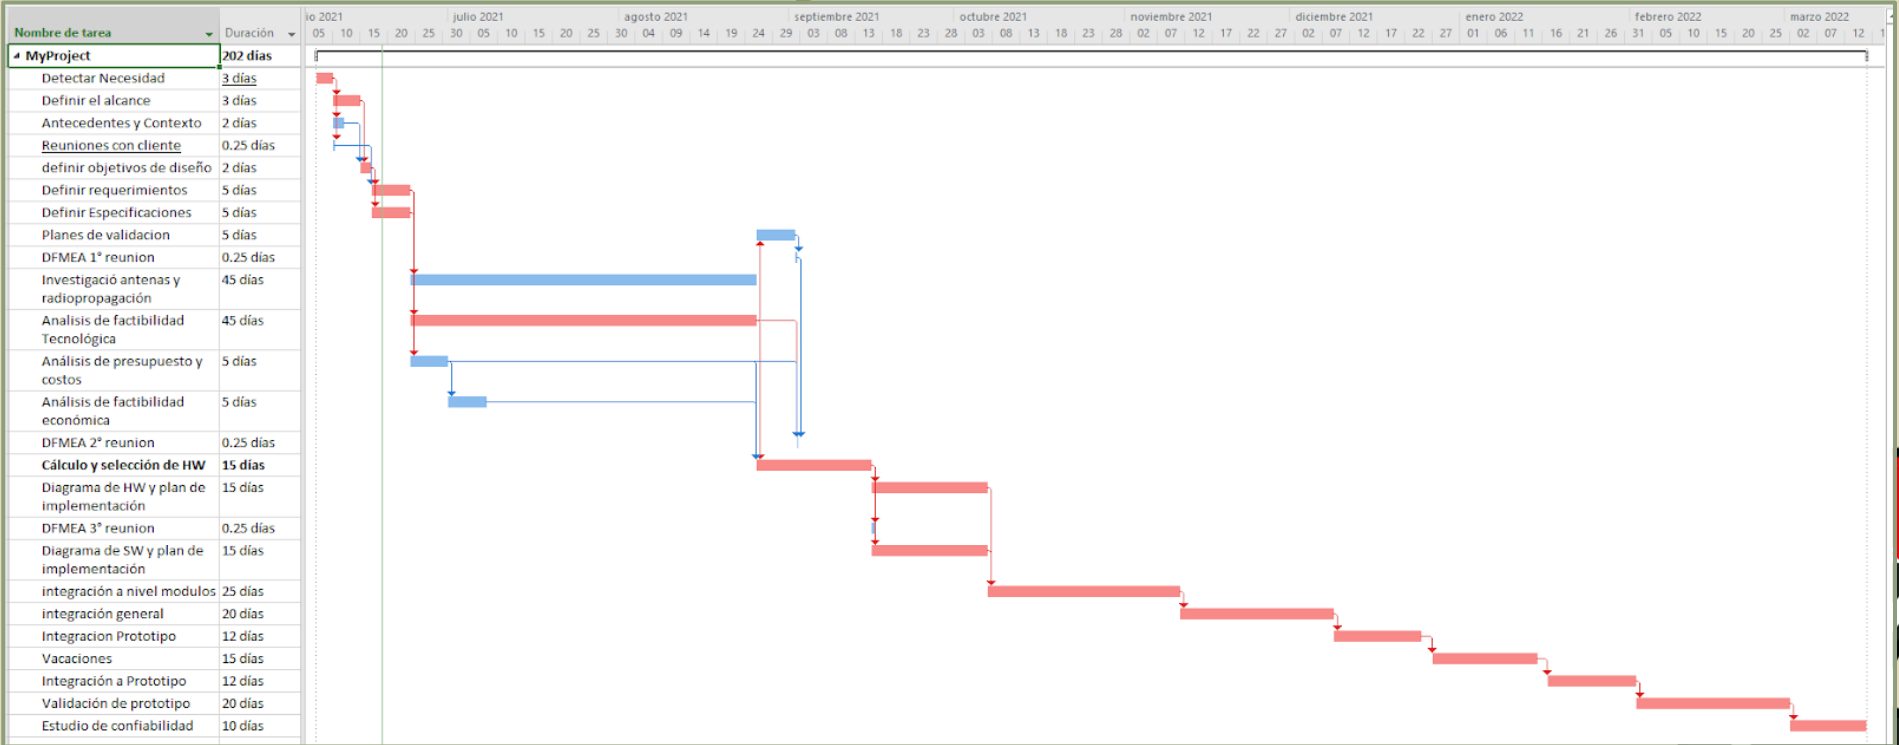
\includegraphics[width=1\linewidth]{ImagenesFactibilidad/project}
	\caption{Diagrama de Gantt del proyecto.}							\label{fig:gantt}
\end{figure}

Luego se realizó una simulación de Montecarlo utilizando la distribución $\beta$ para las variables aleatorias, obteniendo como resultado el análisis plasmado en la Figura (\ref{fig:montecarlo_tiempos}). Se tiene en cuenta que por teorema central del límite la suma de las variables aleatorias $\beta$ convergen a una normal.

En este gráfico se ve la probabilidad de terminar el proyecto en un intervalo de entre 1533 a 1957 horas, con una probabilidad del 95\%. Esta distribución es el lapso entre que se comienza el proyecto y se termina, a través del camino crítico.

\begin{figure}[H]
	\centering
	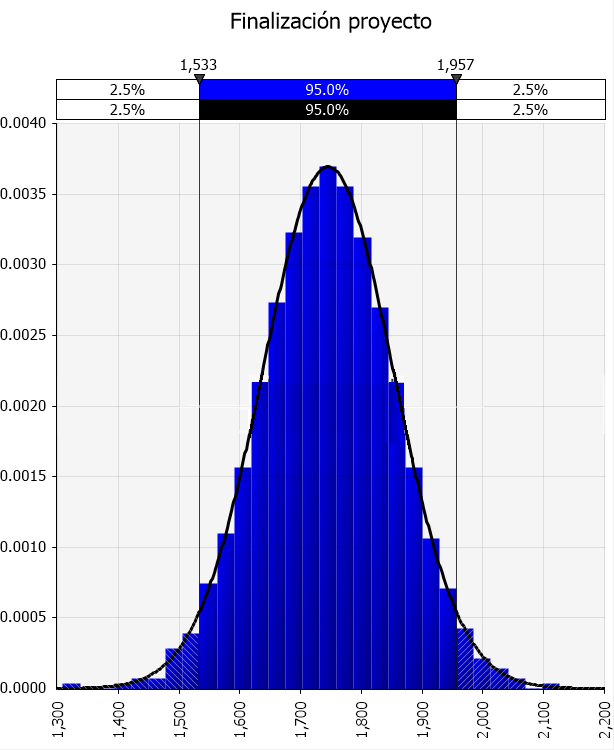
\includegraphics[width=0.5\linewidth]{ImagenesFactibilidad/montecarlo}
	\caption{Simulación de Montecarlo.}	
	\label{fig:montecarlo_tiempos}
\end{figure}


A continuación, se muestran la cantidad de horas de ingeniería total. Para obtener los resultados de la Figura (\ref{fig:montecarlo_tiempos_ing}), se tuvieron cuenta la paralelización de actividades y la disponibilidad de 4 trabajadores.
\begin{figure}[H]
	\centering
	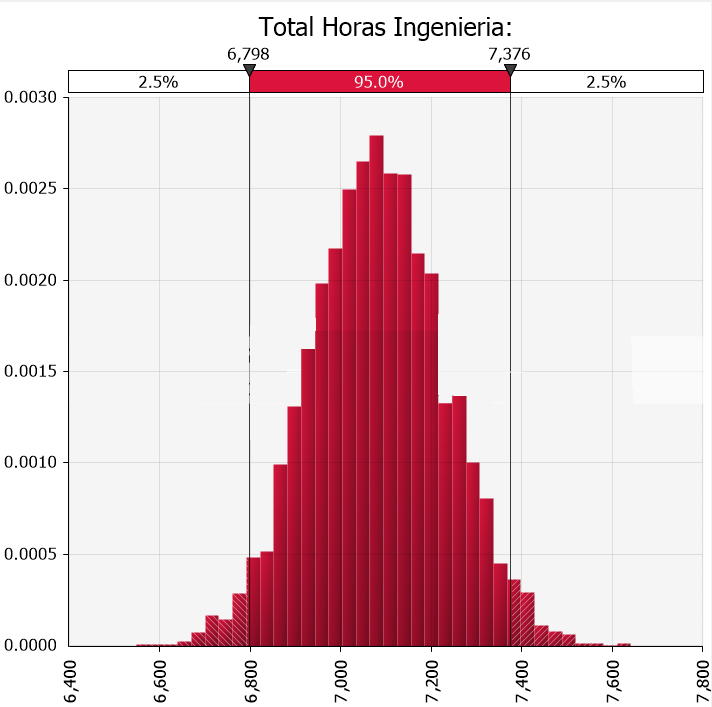
\includegraphics[width=0.5\linewidth]{ImagenesFactibilidad/montecarlo_tiempo_largo}	
	\caption{Simulación de Montecarlo para tiempo de ingeniería.}
	\label{fig:montecarlo_tiempos_ing}
\end{figure}

Se puede observar que el tiempo total de horas de ingeniería corresponde a un rango entre aproximadamente 6800 a 7400 horas, con una media de aproximadamente 7100 horas.

\Subsection{Factibilidad Económica}
%(Mercado, costos, ciclo de vida, %VAN, TIR)
Para poder estudiar la viabilidad financiera de todo emprendimiento es necesario hacer un balance cuidadoso de los diferentes costos en los que se va a incurrir. Se debe analizar cuales serán la fuentes de ingresos que hagan del modelo de negocio planteado un negocio sostenible en el tiempo. 
En este caso en particular estamos analizando el caso de un proyecto único. Sin embargo, no se desea descartar la posibilidad de realizar más unidades en el futuro por fuera del marco del proyecto. Es por esto que presentamos aquí debajo el modelo de negocios planteado para referencia futura. 
\Subsubsection{Modelo de Negocios}

Este diseño se trata de un proyecto único, con posibilidad de realizar hasta \unidadespostfin unidades adicionales posteriores a su finalización. Para dar una visión global se planteo el siguiente modelo de Canvas:
 

\begin{figure}[H]
	\centering
	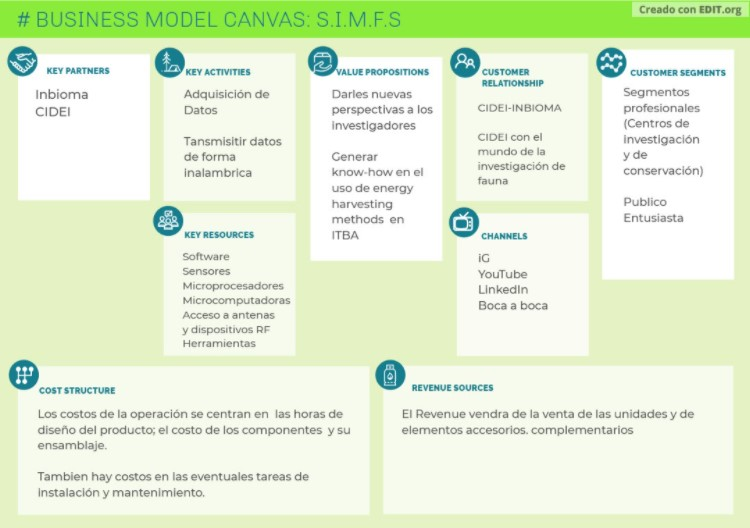
\includegraphics[scale=0.7]{../Factibilidad/ImagenesFactibilidad/ModeloDeCanvas}
	\caption{Modelo de negocio.}
	\label{fig:modelodecanvas}
\end{figure}



\Subsubsection{Investigación y Desarrollo}
Este proyecto contiene una gran componente de diseño. Según lo establecido en la programación del proyecto, el tiempo invertido de diseño esta estimado en 5472 horas. %todas las horas hasta "integracion a nivel modulos" sin incluir
Una vez completada la etapa de diseño el equipo se aboca a la implementación del primer prototipo, es decir a la integración del hardware a utilizar y el desarrollo del software que controla al nido que permite la interacción con el mismo. 

Realizando la estimación sobre un sueldo de $30 \ \frac{USD}{hora}$ y multiplicándolo por la cantidad de horas de ingeniería esperada por persona se obtiene un total de: $$Costo \ mano \ de \ obra = 7100 \ hora \ \cdot 30 \ \frac{USD}{hora} = 213.000,00 \ USD$$


\Subsubsection{Gastos fijos por unidad}

Los gastos principales considerados son USD$254.09$. %Para la compra de los componentes, se suman los costos estimados previamente, más el resto de los componentes misceláneos (resistores, capacitores, etc.) para el diseño de los circuitos involucrados.
%Se estima de este modo un costo de componentes de \TBD USD, a contabilizar una única vez por unidad.

Se presenta el valor de los insumos de hardware y de montaje:
\begin{table}[H]
\centering
\begin{tabular}{|c|c|}
\hline
\textbf{Item}                                                         & \textbf{Precio [USD]}				  \\ \hline
Sensor humedad-temperatura 											  & 4.9                                   \\ \hline
Sensor luminosidad                                                    & $1.54    $                              \\ \hline
M\'odulo RTC                                                     & $2.33$                                  \\ \hline
Cámara                                                                & $20$                                    \\ \hline
SDI 32GBy                                                             & $32$                                    \\ \hline
\rpi 3B
 & $25.5$                                  \\ \hline
Batería                                                               & $86  $                 				  \\ \hline
Panel solar                                                           & $25$ 				  \\ \hline
MPPT                                                                  & $18$                                    \\ \hline
Encapsulado                                                           & $16$                                    \\ \hline
Módulo Bluetooth 5.0                                                           & $3.82 $                                   \\ \hline
Montaje                                                               & $31$                                    \\ \hline
Extras
& $15$									\\ \hline
\textbf{Total}
&\textbf{$254.09$} \\ \hline
\end{tabular}
\caption{Valores de insumos.}
\end{table}


\Subsubsection{Reserva de Contingencia}
Dado que este proyecto cuenta con un alto grado de investigación es necesario contar con un cierto margen de seguridad en caso de que ocurra un cambio de planes necesario para alcanzar el objetivo del proyecto. Es por eso que se decidió incluir en nuestro análisis un adicional del 5\% sobre el costo total del proyecto. Esta suma sera devuelta al cliente en caso de no necesitarla.

La reserva de contingencia se ubicara en  USD 11.000
\Subsubsection{Escenario de Escala}
Se contempla que en el caso de que la producción sea de \unidadespostfin unidades será posible conseguir los insumos necesarios para el ensamblado de las unidades a precio de venta al por mayor.


\Subsection{Factibilidad Legal y Responsabilidad Civil}
\label{sec:legal}
En cuanto a la emisión de ondas electromagnéticas, las normas y regulaciones que se deben considerar son:
\begin{itemize}
	\item Resolución 202/95 (Estándar Nacional de Seguridad para la Exposición a radiofrecuencias comprendidas entre 100 $KHz$ y 300 $GHz$).
	\item Resolución 530/2000 (Estándar Nacional de Seguridad de aplicación obligatoria a todos los sistemas de telecomunicaciones que irradian en determinadas frecuencias).
	\item Resolución 1994/2015 (Regulación SAR).
	\item \textit{Guidelines} de la FCC en exposición máxima recomendada. Una densidad de potencia de 580 $\mu W/{cm}^2$ @ 850 $MHz$.
	\item Ministerio de Salud y Acción Social admite como máxima una densidad de potencia de 450 $\mu W/{cm}^2$ @ 850 $MHz$.
	\item \textit{The Worldwide Approval Status fo}r $900 \ MHz$ \textit{and} $2.4 \ GHz$ \textit{Spread Spectrum Radio Products}. Establece un límite de 4 $W$ para la potencia de la antena transmisora.
\end{itemize}

En lo que a la preservación del medio ambiente respecta, la Ley 26.331 estipula los siguientes aspectos de interés:
\begin{itemize}
	\item Se debe considerar un Plan de Manejo Sostenible de Bosques Nativos.
	\item El Plan debe cumplir las condiciones mínimas de persistencia, producción sostenida y mantenimiento de los servicios ambientales de los bosques.
\end{itemize}

A esto se le suma lo estipulado en la Ley 13.273. En esta se encuentra que se constituye como contravenciones forestales destruir, remover o suprimir señales o indicadores colocados por la autoridad forestal, entre otras cosas.


%\end{document}